\documentclass[lettersize,journal]{IEEEtran} 
\usepackage{bm}
\usepackage{verbatim}
\usepackage{calc}
\usepackage{algorithm2e}
\usepackage{array}
\usepackage{booktabs}
\usepackage{colortbl}
\usepackage{supertabular}
\usepackage{amsmath,amsfonts}
\usepackage{tikz}
\usetikzlibrary{calc}
\usepackage{subfig}
\usepackage{pgfplots} 
\usepackage{pgfplotstable}
\usepgfplotslibrary{patchplots}
\pgfplotsset{compat=1.7}
\usepgfplotslibrary{dateplot}
\hyphenation{op-tical net-works semi-conduc-tor IEEE-Xplore}
\def\BibTeX{{\rm B\kern-.05em{\sc i\kern-.025em b}\kern-.08em
    T\kern-.1667em\lower.7ex\hbox{E}\kern-.125emX}}
\usepackage{balance} 
\usepackage{ifthen}
\makeatletter
\@ifundefined{doPgfSetup}{%
\def\doPgfPlot{true}
\pgfplotsset{
	SmallBarPlot/.style={font=\footnotesize, ybar, width=\linewidth, ymin=0, xmin=0, xmax=1.8, xtick=data, xticklabel style={text width=1.5cm, rotate=0, legend pos=north west, align=center}},
	SmallTimeSeriesPlot/.style={font=\footnotesize, width=\linewidth, height=2in, date coordinates in=x, xticklabel=\hour:\minute, ymin=0, ymax=100, legend pos=north west,
	major grid style={lightgray}, grid=both, minor grid style={lightgray!25}, minor tick num=1},
	SmallPointPlot/.style={font=\footnotesize, width=\linewidth, legend pos=south west, major grid style={lightgray},
	 grid=both, minor grid style={lightgray!25}, minor tick num=1},
	TimeMatrix/.style={font=\footnotesize, width=\linewidth, height=2in, date coordinates in=x, xticklabel=\hour:\minute} 
	}
}
\makeatother

\makeatletter
\@ifundefined{makeComparisonChartLogThree}{%
\newcommand\makeComparisonBarChartLogThree[4]{%
	\pgfplotstableread[col sep=comma]{#1}\table
	\begin{tikzpicture}
		\begin{axis}[SmallBarPlot, xticklabels from table={\table}{type}, ylabel=#2, ymode = log]
			\addplot [fill=blue!20, bar width=0.4] table [x expr=\coordindex*0.6 + 1 - 0.1, y=#3]{\table};
			\addplot [fill=red!20, bar width=0.4] table [x expr=\coordindex*0.6 + 1 + 0.1, y=#4]{\table};
		\end{axis} 
	\end{tikzpicture} 
}
}
\makeatother


\makeatletter
\@ifundefined{makeComparisonBarChartThreeThree}{%
\newcommand\makeComparisonBarChartThreeThree[5]{%
	\pgfplotstableread[col sep=comma]{#1}\table
	\begin{tikzpicture}
		\begin{axis}[SmallBarPlot, xticklabels from table={\table}{type}, ylabel=#2]
			\addplot [fill=blue!20, bar width=0.15] table [x expr=\coordindex*0.6 + 0.3, y=#3]{\table};
			\addlegendentry{#3}
			\addplot [fill=green!20, bar width=0.15] table [x expr=\coordindex*0.6 + 0.3, y=#4]{\table};
			\addlegendentry{#4}
			\addplot [fill=red!20, bar width=0.15] table [x expr=\coordindex*0.6 + 0.3, y=#5]{\table};
			\addlegendentry{#5}
			\legend{#3, #4, #5}
		\end{axis}
	\end{tikzpicture} 
}
}
\makeatother

\makeatletter
\@ifundefined{makeComparisonPowerThree}{%
\newcommand\makeComparisonPowerThree[5]{%
	\pgfplotstableread[col sep=comma]{#1}\firstTable
	\pgfplotstableread[col sep=comma]{#2}\secondTable
	\centering
	\begin{tikzpicture}
		\begin{axis}[SmallTimeSeriesPlot, ymin=-10, ymax=800, xlabel=Time (hr:min), ylabel=#3, legend style={nodes={scale=0.7}}]
			\addplot[blue, smooth] table [x = {time}, y = {meanBusPower}]{\firstTable};
			\addplot[red, smooth] table [x = {time}, y = {meanBusPower}]{\secondTable};
			\addplot[brown, smooth] table [x = {time}, y = {loadPower}]{\firstTable};
			\filldraw[fill=gray!40, opacity=0.3](625,0) rectangle (917,950);
			\addlegendimage{line width=10pt, color=gray!40, draw opacity=0.5}
			\legend{#4, #5, Uncontrolled Load, On-Peak Time}
		\end{axis} 
	\end{tikzpicture} 
}
}
\makeatother

\makeatletter
\@ifundefined{makeComparisonTotalPowerThree}{%
\newcommand\makeComparisonTotalPowerThree[5]{%

\pgfplotstableread[col sep=comma]{#1}\firstTable
\pgfplotstableread[col sep=comma]{#2}\secondTable
\begin{tikzpicture}
	\begin{axis}[SmallTimeSeriesPlot, xlabel=Time (hr:min), ylabel=#3, ymin = -10, ymax=2500, legend style={nodes={scale=0.6}}]
		\filldraw[fill=gray!40, opacity=0.3](625,0) rectangle (917,300);

		\addplot[blue, smooth] table [x = {time}, y = {facilitiesOut}]{\firstTable};
		\addplot[red, smooth] table [x = {time}, y = {facilitiesOut}]{\secondTable};

		\addplot[draw=green!20!black,fill=green!40!cyan!40, mark=pentagon*, only marks, mark size=3pt, y filter/.expression={y==0 ? nan:y}] table [x={time}, y={maxFacilitiesOut}]{\firstTable};
	        \addplot[draw=red,fill=green!10!orange!40, mark=pentagon*, only marks, mark size=3pt, y filter/.expression={y==0 ? nan:y}] table [x={time}, y={maxOnPeakOut}]{\firstTable};

		\addlegendimage{line width=10pt, color=gray!40, draw opacity=0.5}; 
	        \addplot[draw=green!20!black,fill=green!40!cyan!40, mark=pentagon*, only marks, mark size=3pt, y filter/.expression={y==0 ? nan:y}] table [x={time}, y={maxFacilitiesOut}]{\secondTable};
		\addplot[draw=red,fill=green!10!orange!40, mark=pentagon*, only marks, mark size=3pt, y filter/.expression={y==0 ? nan:y}] table [x={time}, y={maxOnPeakOut}]{\secondTable};   

	        \legend{#4, #5, Maximum Overall Average Power, Maximum On-Peak Average Power, On-Peak Time};
	\end{axis} 
\end{tikzpicture}

}
}
\makeatother




\usepackage[backend=bibtex, style=numeric, sorting=none]{biblatex}
\def\rootdirectorythree{.}
\bibliography{references}
\begin{document} 
\title{A Scalable Approach to Minimize Charging Cost for Electric Bus Fleets}
\author{Daniel Mortensen, Jacob Gunther\thanks{}}

\markboth{Transactions on Intelligent Transportation Systems}%
{}

\maketitle 
\begin{abstract}
Encorporating battery electric buses into bus fleets faces three primary challenges: a BEB's extended refuel time, the cost of charging, both by the consumer and the power provider, and large compute demands for planning methods. When BEBs charge, the additional demands on the grid may exceed hardware limitations and so power providers divide a consumer's energy needs into separate meters even though doing so is expensive for both power providers and consumers. Prior work has developed a number of strategies for computing charge schedules for bus fleets, however prior work has not worked to reduce cost by aggregating meters. Additionally, because many works use mixed integer linear programs, their compute needs make planning for commercial sized bus fleets intractable. This work presents a multi-program approach to computing charge plans for electric bus fleets. Rather than posing a single large MILP that incorporates every aspect of the charging problem, we solve a series of small subproblems in which the solution to the charging problem becomes successively more refined and moves closer to the optimal schedule. Our results show that intermediate subproblems can be solved with a dramatic reduction in runtimes allowing our method to be applied to significantly larger bus fleets. In fact, we will show that not only do the runtimes scale linearly with the number of buses, easily planning for fleets of 100+ buses, but the monthly cost does as well.
\end{abstract}

\begin{IEEEkeywords}
Battery Electric Bus, Charge Schedule, Mixed Integer Linear Program, Bus Fleet, Grid Management
\end{IEEEkeywords}

\section{Introduction}
\par  Many transit authorities desire to use battery electric buses (BEBs) for public transportation because BEBs offer many benefits \cite{Mahmoud2016} including reduced maintenance \cite{poornesh_comparative_2020}, zero emissions \cite{kato_comparative_2013}, and access to renewable energy \cite{cheng_smart_2020}.
\par Unfortunately, BEBS cannot replace traditional buses without managing lengthy charge times. Historically, a bus using diesal or comparessed natural gas (CNG) refuels quickly so that fuel times play a minor role in their use. However charge times for BEBs can range up to several hours, which presents logistical challenges for bus fleets and necessitate detailed charge plans which address four points of interest: battery state, bus availability, charging resources, and the cost of using electrical infrastructure. 
\par Addressing battery state includes charging buses so that their state of charge remains above a minimum threshold. Futhermore, if computations are only done for one day, the state of charge for each bus at the end of the day must be the same as the beginning. Constraints for bus availability only allow charging when buses are near charging resources. 
\par For example, if all chargers are located at the bus station, then each bus's availability would mirror its time in the station. Unfortunately, proximity to charging resources alone does not gaurentee access because other buses may already occupy the chargers. 
\par Finally, when a bus does gain charger access, power providers assess charges for both energy and power so that high charge rates quickly become expensive. High charge rates are not limited to single buses either as the power and energy for each bus is combined at a single meter including loads that are not related to bus charging. For example, if two buses charged at 200 kW each, and an additional non-bus load drew 100 kW, then the power provider would assess a power charge based on 500 kW of use. In this work, we refer to the problem of forming a charge plan under the aforementioned constraints as the ``charge problem''.
\section{Previous Work}
\par The charge problem has received attention in previous work and is generally addressed in one of three ways: dynamic charging, battery swaps, and static charging.
\subsection{Dynamic charging}
\par Dynamic charging allows buses to utilize charging resources while in motion, generally through overhead charging lines \cite{csonka_optimization_2021}, or inductive power transfer \cite{jeong_automatic_2018} \cite{balde_electric_2019}. 
\par Dynamic charging increases access to charging resources because buses can refuel while in motion so that availability does not depend on time spent in the bus station. Unfortunately, both overhead and inductive chargers require additional hardare; overhead chargers through the overhead power lines, and inductive charging through specialized hardware beneath the road. Both of which require additional infrastructure \cite{Alwesabi_2022_Robust} which may be unavailable, or cost prohibitive.
\subsection{Battery Swaps}
\par Battery swaps manage the energy needs for each bus by replacing spent batteries so that they can be charged without delaying the buses as proposed by \cite{jain_battery_2020} and \cite{xian_zhang_optimal_2016}. Battery exchanges greatly simplify charge plans and relieve the need for dynamic infrastructure. The only drawback to battery swaps comes from how BEBs are constructed as BEBs are not built to exchange batteries. Therefore, the task can require specialized hardware, technical expertise, or automation.
\subsection{Static Charging}
\par A static charging scenario takes place when charging resources remain anchored so that buses must stop in order to refuel and is the least invasive way to manage a bus fleet's energy needs. Prior work in this area addresses a number of problems, including distributed charging networks \cite{Nimalsiri2020}, bus availability, environmental impact \cite{zhou_bi-objective_2021}, route scheduling \cite{Rinalde_Mixed_2020}, battery health \cite{houbbadi_optimal_2019}, the cost of electricity \cite{Leou_optimal_2017}, and the cost of charging infrastructure \cite{Wei2018}.
\par Because charge times can be lengthy, some prefer to use high power chargers, which deliver more energy in a smaller period of time. However doing so places large power demands on electrical infrastructure \cite{stahleder_impact_2019} so that power networks becomes unreliable \cite{deb_impact_2017} and expensive because high power requires additional maintenance and upgrades \cite{boonraksa_impact_2019}. An effective charge plan must therefore balance the need to charge quickly with the desire to maintain a low power profile \cite{ojer_development_2020}.
\par Methods for developing a charge plan range from heuristic approaches \cite{qin_numerical_2016} \cite{Wang2019} to globally optimal solutions, generally through mixed integer linear programs (MILP) \cite{bagherinezhad_spatio-temporal_2020}, where the first prioritizes computational time and the second focuses on cost. Generally, each method minimizes cost by either decreasing the instantaneous power needs for the fleet, or optimizing over time of use tarrifs \cite{He_2019_Fast}.  
\subsection{Contributions}
\par  This work extends previous methods with two primary contributions: Uncontrolled loads, and scalability for both computation time and cost. Uncontrolled loads are defined as non-BEB loads which impact monthly cost. For example, the Utah Transit Authority in Salt Lake City manages several loads including an electric train, a station for compressed natural gas (CNG), and electric buses. 
\par When the train arrives at the station, the regenerative brakes input power to the grid, which would complement high charge rates on a BEB charger. However the train requires significant power to accelerate and makes additional charging unwise when it departs\par Generally, previous work falls into one of two categories. The first prioritises computation time at the expense of cost, generally through heuristics. The second finds a globally optimal solution, but does so at the cost of computation time. This paper presents a method which accounts for both so that computation time and monthly cost increase linearly with the number of buses. 

\section{$p_1$: Unconstrained Schedule \label{sec:unconstrainedSchedule}}
This section describes a program that solves $p_1$ by finding an optimal charge schedule where buses are allowed to charge without regard to the number of available chargers. This solution is considered ``optimal'' and will be used in later sections to formulate a feasible solution that accounts for the number of chargers.
\begin{table*}
\centering
\caption{Description of the billing structure}
\begin{tabular}{c | c c c}
		                   & On-Peak                & Off-Peak               & Facilities (Both)\\ \hline
		Energy Rate        & \$ 0.058282  /kWh & \$ 0.029624 /kWh  & None \\
		Energy Rate Symbol & $\mu_{\text{e-on}}$    & $\mu_{\text{e-off}}$   & None \\ \hline
		Power Rate  & \$ 15.73 /kW           & None                   & \$ 4.81 /kW \\
		Power Rate Symbol  & $\mu_{\text{p-on}}$    & None            & $\mu_{\text{p-all}}$
	\end{tabular}
	\label{tab:charges} 
\end{table*}

 
\begin{figure*}
\centering
\scalebox{0.8}{
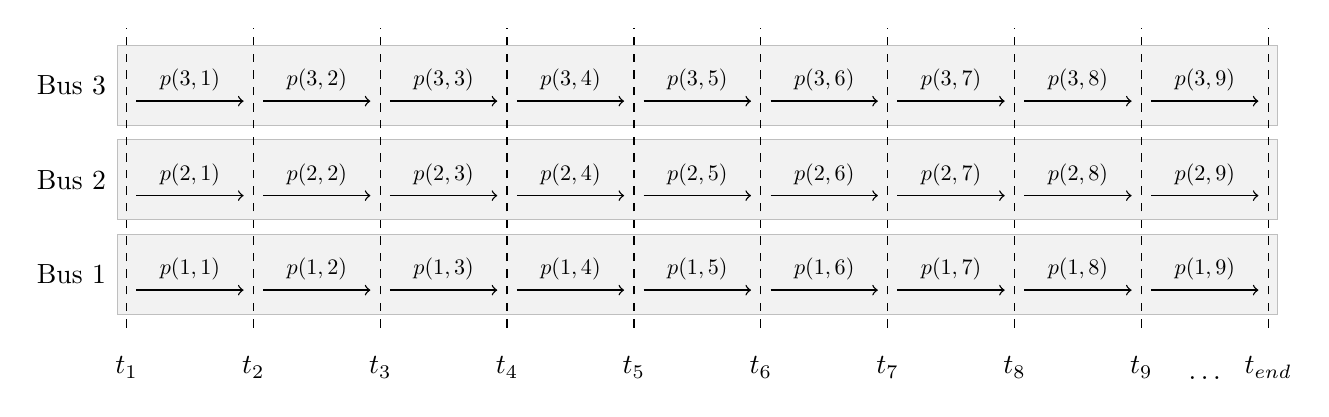
\begin{tikzpicture}
	\node[rectangle, draw=gray!50, fill=gray!10, minimum width=5.8in, minimum height=0.4in](bus1Box) at (7.75,0.8){};
	\node(bus1BoxLabel) at (-0.2, 0.8){Bus 1}; 
	
	\node[rectangle, draw=gray!50, fill=gray!10, minimum width=5.8in, minimum height=0.4in](bus2Box) at (7.75,2){};
	\node(bus1BoxLabel) at (-0.2, 2.0){Bus 2};
	
	\node[rectangle, draw=gray!50, fill=gray!10, minimum width=5.8in, minimum height=0.4in](bus3Box) at (7.75,3.2){};
	\node(bus1BoxLabel) at (-0.2, 3.2){Bus 3};
	
	\foreach \curLab/\preLab[count=\c, evaluate=\c as \pos using {0.5 + (\c - 1)*14.5/9}] in {t_1/t_1, t_2/t_1, t_3/t_2, t_4/t_3, t_5/t_4, t_6/t_7, t_7/t_6, t_8/t_7, t_9/t_8, t_{end}/t_9}
	{
		\node[label=below:$\curLab$](b\c) at (\pos, 0){};
		\node(t) at (\pos, 3.8){};
		\draw[dashed, line width=0.5pt] (b\c.north) -- (t.north); 
		\ifnum\c>1 
			\node(b1Curr) at (\pos, 0.8 - 0.2){};
			\node(b2Curr) at (\pos, 2.0 - 0.2){};
			\node(b3Curr) at (\pos, 3.2 - 0.2){};
			\def\temp{\number\numexpr\c - 1}
			\draw[->, line width=0.5pt] (b1Prev.east) -- node[midway, above]{\scalebox{0.8}{$p(1,\temp)$}}(b1Curr.west);
			\draw[->, line width=0.5pt] (b2Prev.east) -- node[midway, above]{\scalebox{0.8}{$p(2,\temp)$}}(b2Curr.west);
			\draw[->, line width=0.5pt] (b3Prev.east) -- node[midway, above]{\scalebox{0.8}{$p(3,\temp)$}}(b3Curr.west);	
		\fi
			\node(b1Prev) at (\pos, 0.8 - 0.2){};
			\node(b2Prev) at (\pos, 2.0 - 0.2){};
			\node(b3Prev) at (\pos, 3.2 - 0.2){};	
	}
	\path (b9.south) -- node[midway, below=0.1in]{$\hdots$}(b10.south);

\end{tikzpicture}}
\caption{Demonstrates how bus power use is conceptualized}
\label{fig:busPower}
\end{figure*}


\begin{figure*}
\centering
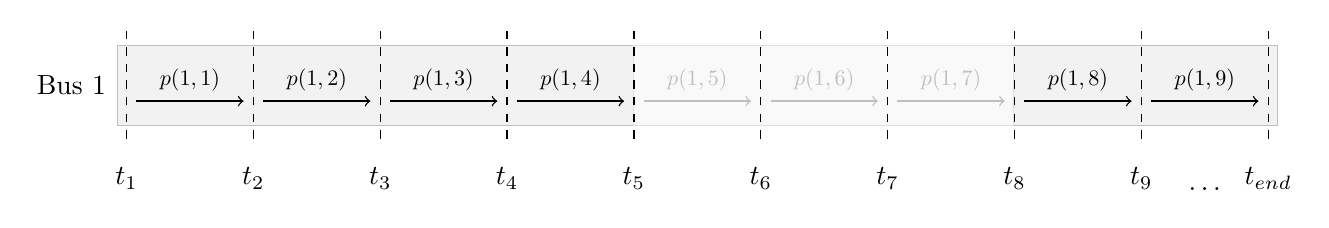
\begin{tikzpicture}
	\node[rectangle, draw=gray!50, fill=gray!10, minimum width=5.8in, minimum height=0.4in](bus1Box) at (7.75,0.8){};
	\node(bus1BoxLabel) at (-0.2, 0.8){Bus 1}; 
	\node[rectangle, draw=gray!25, fill=gray!5, minimum width=1.9in, minimum height=0.4in](bus1Box) at (7.75 + 1.6,0.8){};
	
	\foreach \curLab/\preLab[count=\c, evaluate=\c as \pos using {0.5 + (\c - 1)*14.5/9}] in {t_1/t_1, t_2/t_1, t_3/t_2, t_4/t_3, t_5/t_4, t_6/t_5, t_7/t_6, t_8/t_7, t_9/t_8, t_{end}/t_9}
	{
		\node[label=below:$\curLab$](b\c) at (\pos, 0){};
		\node(t) at (\pos, 1.4){};
		\ifnum\c>1 
			\node(b1Curr) at (\pos, 0.8 - 0.2){};
				\ifnum\c > 5
					\ifnum\c < 9 
						\def\clr{black!25}
					\else
						\def\clr{black}
					\fi
				\else
					\def\clr{black}
				\fi
				\draw[->, line width=0.5pt, \clr] (b1Prev.east) -- node[midway, above]{\scalebox{0.8}{$p(1,\number\numexpr\c-1)$}}(b1Curr.west); 
		\fi
		\node(b1Prev) at (\pos, 0.8 - 0.2){};
		\draw[dashed, line width=0.5pt] (b\c.north) -- (t.north); 
	}
	\path (b9.south) -- node[midway, below=0.1in]{$\hdots$}(b10.south);

\end{tikzpicture}
\caption{Bus schedule with availability}
\label{fig:busAvail}
\end{figure*}

 
\subsection{Formulation \label{sec:formulation}} 
The cost objective we minimize is based on the rate schedule from \cite{rocky_mountain_power_rocky_2021}, which contains two primary elements: the cost of energy, and power demand. Energy is billed per kWh for on-peak and off-peak hours. The on-peak rate is more expensive because there is generally more demand for power during this time, whereas off-peak hours tend to be less expensive. The demand is covered in two separate chargers.  The first is a facilities charge which is billed per kW for the highest 15-minute average power use over the course of the month. The second is a demand charge, which is also billed per kW, but is only billed for the highest 15-minute average power usesd during on-peak hours. The rates for each component are given in Table \ref{tab:charges}.  

Before we may compute the total monthly cost of electricity, we must define expressions for the average power and energy over time.  Let each day be divided into time intervals of length $\Delta T$ for each bus where the average power expended for bus $i$ during time $j$ is denoted $p(i,j)$ as shown in Fig. \ref{fig:busPower} (Note that $\Delta T$ may not be 15 minutes, and expressions for the 15-minute average will be computed later). The resulting solution of $p_1$ will yield the average power expended by each bus during each period of time.
\par One constraint for which the solution must account is bus availability.  When a bus is out of the station, the maximum average power for that time must be zero. For example, if bus 1 were out on route for $t_5, t_6,$ and $t_7$, then the average power for those periods would be equal to zero as shown in Fig. \ref{fig:busAvail}. Let $\bm{b}_{p(i,j)}$ be the average power used by bus $i$ at time index $j$, and $\bm{b}$ be a vector which contains $b_{p(i,j)}$ for each bus and time index. Also let $\mathcal{A} \subset {i\times j}$  be the set of all indices where bus $i$ is in the station during time $t_j$ and $\tilde{\mathcal{A}}$ be its complement. Furthermore, let $p_{\text{max}}$ be the maximum power that a charger can deliver. 
\par We define a set of constraints so that buses do not use power when not in the station by letting
\begin{equation}\label{eqn:obj:power2}\begin{aligned}
	b_{p(i,j)} &= 0 \ \forall i,j \in \tilde{\mathcal{A}}  \\
	b_{p(i,j)} &\le p_{\text{max}} \ \forall i,j \in \mathcal{A} \\
	-b_{p(i,j)} &\le 0              \ \forall i,j \in \mathcal{A} 
\end{aligned}\end{equation}


\subsection{Battery}
\par Each bus must also maintain its state of charge above acceptable levels throughout the day.  When buses leave the station, each bus discharges some quantity of energy throughout the course of the route. Let $\delta(i,j)$ be the amount of charge lost by bus $i$ at time $j$ and let $h(i,j)$ be the state of charge of bus $i$ at time $j$. The state of charge for each bus can be defined as
\begin{equation}\label{eqn:battery:socPropagation}\begin{aligned}
	h(i,j) &= h(i,j-1) + b_p(i,j - 1)\cdot \Delta T - \delta(i,j) \ \forall i,j>1 \\
	h(i,1) &= \eta_i \ \forall i
\end{aligned}\end{equation}
where $\eta_i$ is the initial state of charge for bus $i$ and $\Delta T$ is the difference in time between $t_{i,j}$ and $t_{i,j+1}$.
Now that each value for the state of charge is defined, each value for $h$ must be constrained so that it is greater than a given threshold, $h_{\text{min}}$ but does not exceed the maximum battery capacity $h_{\text{max}}$. This yields
\begin{equation} \label{eqn:battery:soc}\begin{aligned}
	-h(i,j) &\le -h_{\text{min}}\ \forall i,j \\
	h(i,j) &\le h_{\text{max}} \ \forall i,j. 
\end{aligned}\end{equation}
\par The final battery related constraint has to do with how we are planning for the bus.  The expenses that come from power are computed monthly, but we desire to simulate the movements of the bus for only a day, and use this to extrapolate what the monthly cost may be.  Therefore, the state of charge for a bus at the end of the day must reflect its starting value.  This yields the following constraint:
\begin{equation}\label{eqn:battery:busPower}
	h_{i,\text{end}} = h(i,1) \ \forall i.
\end{equation}


\subsection{Cumulative Load Management}
\par While this formulation does not directly account for the number of available chargers, we do account for the cumulative load capacities of all chargers.  Let the number of chargers be denoted $n_{\text{charger}}$. We desire to maintain the average cumulative power for each time step at a level that is serviceable given $n_{\text{charger}}$. We define a slack variable $p_c(j)$ which represents the total average power consumed by all buses at time $j$.  The variable $p_c(j)$ is computed as the sum of average bus powers so that
\begin{equation}\label{eqn:cumulative:power}
	p_c(j) = \sum_ib_{p(i,j)}.
\end{equation}

\subsection{Objective\label{sec:objective}}

\par Now that the relevent constraints have been addressed, we turn attention to the objective function. We start by computing the total average power for the complete system. This total power is comprised of power used by the buses, and power used by external sources such as lights, ice melt, electric trains, etc which we refer to as ``uncontrolled loads'', where the average power for the uncontrolled loads at time step $j$ is denoted $u(j)$. We compute the total power as the sum of power used by the buses, $p_c(j)$ and the power consumed by uncontrolled loads $u(j)$ so that the total power, denoted $p_t(j)$ is computed as 
\begin{equation}\label{eqn:objective:pt}
	p_t(j) = p_c(j) + u(j).
\end{equation}
      
\par The next step is to compute the fifteen minute average power use for each time step, denoted $p_{\text{15}}$. We do this by letting 
\begin{equation}\label{eqn:objective:p15}
p_{\text{15}}(j) = \frac{1}{n}\sum_{l \in \{j_{15}\}}p_t(l)
\end{equation}
where $\{j_{15}\}$ is the set of all indices 15 minutes prior to time $t_j$ and $n$ is the cardinality of $\{j_{15}\}$.
Next, note that the rate schedule requires both the maximum overall average power, denoted $p_{\text{facilities}}$, and the maximum average power during on-peak hours, or $p_{\text{demand}}$. Let $\mathcal{S}_{\text{on}}$ be the set of time indices belonging to on-peak hours, and recall that the max over all average power values is greater than or equal to $p_{15}(j)$ for all $j$. We can express this constraint as
\begin{equation}\label{eqn:objective:pFac}
	p_{\text{facilities}} \ge p_{15}(j) \ \forall j.
\end{equation}
Because $p_{\text{facilities}}$ will be used in the objective function, the value for $p_{\text{facilities}}$ will be minimised until it is equal to the largest value in $p_{15}$. Following a similar logic, we also define a set of constraints for the maximum average on-peak power, $p_{\text{demand}}$ so that
\begin{equation}\label{eqn:objective:pDem}
	p_{15}(i) \leq p_{\text{demand}} \ \forall i \in \mathcal{S}_{\text{on}}.
\end{equation}
The next step in computing the objective function is to compute the total {\it energy} consumed during on and off-peak hours respectively.  Let $e_{\text{on}}$ be the total energy consumed during on-peak hours and $e_{\text{off}}$ be the energy consumed during off-peak hours. We can compute energy as the product of average power and time.  In our case, we compute this as 
\begin{equation}\label{eqn:objective:energy}\begin{aligned}
	e_{\text{on}} &= \Delta T\cdot \sum_{i \in \mathcal{S}_{\text{on}}}p_t(i) \\ 
	e_{\text{off}} &= \Delta T\cdot \sum_{i \notin \mathcal{S}_{\text{on}}}p_t(i).  
\end{aligned}\end{equation}
We can now compute the total monthly cost in dollars as
\begin{equation}\label{sec:unconstrainedSchedule:objective}
J_{\text{cost}} = \begin{bmatrix}e_{\text{on}} \\ e_{\text{off}} \\ p_{\text{facilities}} \\ p_{\text{demand}} \end{bmatrix}^T \begin{bmatrix} \mu_{\text{e-on}} \\ \mu_{\text{e-off}} \\ \mu_{\text{p-all}} \\ \mu_{\text{p-on}} \end{bmatrix} 
\end{equation}

\par The final optimization problem that computes a charge schedule without constraints on the number of chargers is descibed below.\\[0.1in]
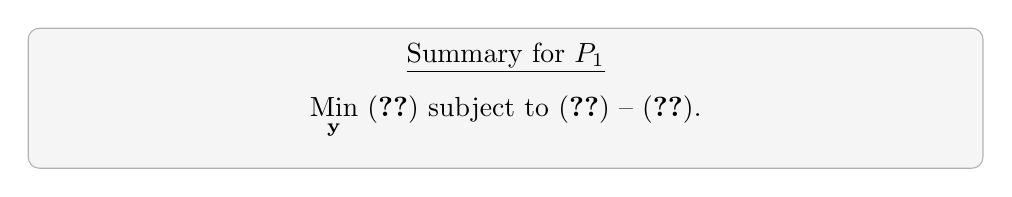
\begin{tikzpicture}
	\node[rectangle, rounded corners, fill=gray!8, draw=gray!60, minimum width=\columnwidth, minimum height=0.7in] at (0,0)(box){};
	\node at (0,0.2in)(title){\underline{Summary for $P_1$}};
	\node at ($(box.south)!0.6!(title.south)$)(text){$ 
	\underset{\mathbf{y}}{\text{Min}}  \ \eqref{sec:unconstrainedSchedule:objective} \  \text{subject to} \ \eqref{eqn:obj:power2} \ \text{--} \ \eqref{eqn:objective:energy}.% \ \eqref{eqn:battery:socPropagation}, \ \eqref{eqn:battery:soc}, \ \eqref{eqn:battery:busPower}, \ \eqref{eqn:cumulative:power}, \ \eqref{eqn:objective:pt}, \ \eqref{eqn:objective:p15}, \ \eqref{eqn:objective:pFac}, \ \eqref{eqn:objective:pDem}, \ \eqref{eqn:objective:energy}
$};
\end{tikzpicture}

\par We have observed that charge commands in solutions to $P_1$ tend to switch frequently between $0$ and $p_{\text{max}}$, which is difficult to implement in practice and imparts stress on charging hardware. Before additional steps can be taken, a smoother set of charge commands is computed, and this is the subject of the next section.

\section{$P_2$: Unconstrained Smooth Schedule \label{sec:unconstrainedSmoothSchedule}}

\par This section implements a smoothing criteria so that the frequent ``on-off'' switching patterns from $P_1$ are reduced. This is done by modifying $P_1$ in two ways. The first is that the demand, facilities, on-peak energy, and off-peak energy are removed from the objective and constrained to equal their values obtained in the solution to $P_1$ so that
\begin{equation}\label{eqn:unconstrainedSmooth:equivalence}\begin{aligned}
	e_{\text{on}} &= \tilde{e}_{\text{on}} \\
	e_{\text{off}} &= \tilde{e}_{\text{off}} \\
	p_{\text{facilities}} &= \tilde{p}_{\text{facilities}} \\
	p_{\text{demand}} &= \tilde{p}_{\text{demand}},
\end{aligned}\end{equation}
where values on the right-hand side are constants extracted from the solution to $P_1$.
Next, we define an alternative objective that incentivizes continuity of charging between time steps. This objective is defined as
\begin{equation}\label{eqn:objective:smooth}
	J_{\text{switch}} = \frac{1}{n}\sum_{i,j, \in \mathcal{K}}\lVert b(i,j) - b(i,j-1) \rVert^2_2,
\end{equation}
where $\mathcal{K}$ is the set of all $i,j$ where bus $i$ may charge during time $j$ and $j - 1$.  The final optimization problem that produces smooth charging schedules is given below.\\[0.1in]
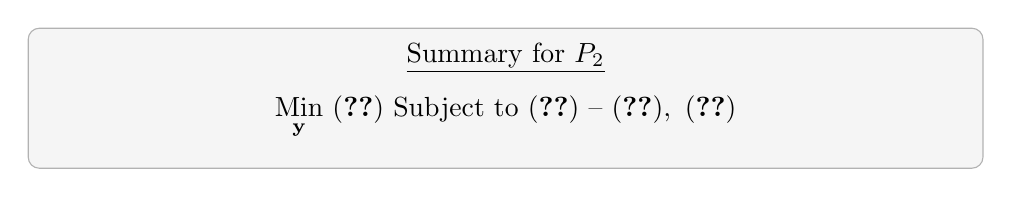
\begin{tikzpicture}
	\node[rectangle, rounded corners, fill=gray!8, draw=gray!60, minimum width=\columnwidth, minimum height=0.7in] at (0,0)(box){};
	\node at (0,0.2in)(title){\underline{Summary for $P_2$}};
	\node at ($(box.south)!0.6!(title.south)$)(text){$ 
	\underset{\mathbf{y}}{\text{Min}} \ \eqref{eqn:objective:smooth} \ \text{Subject to} \ \eqref{eqn:obj:power2} \ \text{--} \ \eqref{eqn:objective:energy}, \ \eqref{eqn:unconstrainedSmooth:equivalence}
$};
\end{tikzpicture}

\par The solution to $P_2$ smooths charge schedules without increasing costs, but it presents the undesireable feature that the charge sessions tend to be fragmented into many short sessions. Additionally, the schedule does not account for the number of chargers or bus contention for charger use. Unfortunatly, addressing these problems requires the use of binary variables and optimization with binary variables becomes untractable for large numbers of buses and chargers. Before the fragmentation and charger assignment problems can be addressed, we first segment the buses into groups.  Successive processing can be done separately in groups which helps to manage the computational complexity for later problems that incorporate binary variables.

\section{$P_3$: Group Assignment\label{sec:groupAssignment}}
This section addresses the matter of problem size.  An optimization problem for scheduling must evaluate all possible combinations of bus-to-charger assignments to select an optimal, contention-free schedule. Because contention increases on the order of $O(n^2)$ with the number $n$ of charge sessions and requires that each combination be evaluated to find an optimal solution, the assignment problem is NP-hard \cite{kolesar_branch_1967}. {\textbf [I don't think $n^2$ is NP-hard.  It's just hard.]} Before we can formulate a scalable solution to the bus problem, we propose a method to separate buses into groups to reduce the coupling between charge sessions.
\par The group assignment problem separates buses into $n_{\text{group}}$ groups, where group $m$ is allocated $n^m_{\text{charger}}$ chargers and $n^m_{\text{bus}}$ buses. Each group must have sufficient chargers to fill its needs and prefer buses with dissimilar schedules to better avoid contention. 
We know that the number of cross-terms in future problems will be reduced when each group has the same number of buses. Therefore, let $n^m_{\text{bus}}$ be described as
\begin{equation}\label{eqn:groups:nBusPerGroup}\begin{aligned}
	n^m_{\text{bus}} &\ge \left \lfloor \frac{n_{\text{bus}}}{n_{\text{group}}} \right \rfloor \\
	n^m_{\text{bus}} &\le \left \lceil \frac{n_{\text{bus}}}{n_{\text{group}}} \right \rceil,
\end{aligned}\end{equation}
where the values $n_\text{bus}$ and $n_\text{group}$ are user parameters.
\par The number of chargers assigned to each group must be exactly equal to the number of available chargers so that
\begin{equation}\label{eqn:groups:nTotalCharger}
	n_{\text{charger}} = \sum_mn_{\text{charger}}^m.
\end{equation}
\par The next set of constraints ensures that each bus is is part of a group exactly once. Let $\beta(i,m)$ be a binary variable which is one when bus $i$ is in group $m$. Each bus is constrained to be a member of exactly one group by letting
\begin{equation}\label{eqn:groups:groupId}
	\sum_m\beta(i,m) = 1 \ \forall i.
\end{equation}
\par We must also ensure that buses are assigned to groups where the power delivered to each bus can be achieved with the number of chargers assigned to that group. Define a slack variable that gives the total power used in group $m$ at time step $j$ as $p(m,j)$. Recall, we also know the expected power use for each bus as this is a result of $P_1$ as $b_{p(i,j)}$, which allows us to describe the total power for any one group as
\begin{equation}\label{eqn:groups:groupPower}
 p(m,j) = \sum_i\beta(i,m)b_{p(i,j)}.
\end{equation}
\par Next, we know that the total load of each group must be less than or equal to the collective capability of that group's chargers, which can be expressed as
\begin{equation}\label{eqn:groups:chargeLimit}
	n^m_{\text{charger}}\cdot p_{\text{max}} \ge p(m,j) \ \forall m,j
\end{equation}
so that the number of chargers is sufficient to charge the collective load of the group. 
\par We also desire to group together buses whos routes have the least overlap. If two buses contain no overlap, they will be easiest to schedule on the same charger.  The overlap is measured using the inner product of their schedules from $P_1$.  If completely non-overlapping, the inner product will be equal to zero. Let
\begin{equation*}
\phi(i,i') = \mathbf{b}(i,:)^T\mathbf{b}(j,:),
\end{equation*}
where $\mathbf{b}(i,:)$ is the charge schedule for bus $i$ as computed in the $P_1$. We desire to minimize the total cross terms $\phi(i,i')$ for all buses in the same group.  Define a slack variable $v(i,i',m)$ which is equal to $\phi(i,i')$ if buses $i$ and $i'$ are both in group $m$ and zero otherwise so that
\begin{equation*}
	\begin{cases}
		v(i,i',m) = \phi(i,i') & \beta(i,m) = 1, \beta(i',m) = 1 \\
		v(i,i',m) = 0 & \text{otherwise}
	\end{cases}
\end{equation*}
which can also be expressed by letting
\begin{equation}\label{eqn:groups:innerProd}\begin{aligned}
	v(i,i',m) &\le \phi(i,i') \\
	v(i,i',m) &\ge \phi(i,i') - M\left (2 - \beta(i,m) - \beta(i',m)\right ) \\
	v(i,i',m) &\le 0 + M\beta(i,m) \\
	v(i,i',m) &\le 0 + M\beta(i',m) \\
	v(i,i',m) &\ge 0.
\end{aligned}\end{equation}
The final objective can then be expressed as
\begin{equation}\label{eqn:groups:objective}
	J_{\text{select}} = \sum_{i,i',m} v(i,i',m).
\end{equation}
The final optimization problem may be expressed as shown below. \\[0.1in]
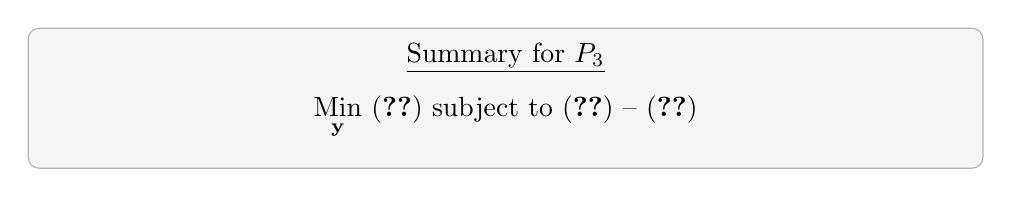
\begin{tikzpicture}
	\node[rectangle, rounded corners, fill=gray!8, draw=gray!60, minimum width=\columnwidth, minimum height=0.7in] at (0,0)(box){};
	\node at (0,0.2in)(title){\underline{Summary for $P_3$}};
	\node at ($(box.south)!0.6!(title.south)$)(text){$ 
	\underset{\mathbf{y}}{\text{Min}} \ \eqref{eqn:groups:objective} \ \text{subject to} \ \eqref{eqn:groups:nBusPerGroup} \ \text{--} \ \eqref{eqn:groups:innerProd} % \ \eqref{eqn:groups:nTotalCharger}, \ \eqref{eqn:groups:groupId}, \ \eqref{eqn:groups:groupPower}, \ \eqref{eqn:groups:chargeLimit}, \ \eqref{eqn:groups:innerProd}
$};
\end{tikzpicture}
\par Problems $P_1$ through $P_3$ have produced preliminary estimates for charge schedules as well as groups into which the buses can be subdivided but have not addressed the problem of fragmentation, where each bus's schedule contains many short charge sessions, whereas fewer charge sessions is desirable. Before we can address where buses should charge, we must first finalize each bus's charge schedule by decreasing the number of charge events.

\section{$p_4$: De-Fragmentation\label{sec:defragmentation}}
A minimum charge session length is another operational constraint that must be considered. We also consider constraints on minimum energy delivered per session. The intent of these constraints is to avoid charging for small durations or for small amounts of energy so that charge sessions are consolidated for convenience. 
\par To solve this program, assume there exists a ``smoothed'' solution from $p_2$ which has been appropriately placed in a group from $p_3$. Next, let the preliminary solution be subdivided into charge sessions, each with a specific amount of energy, a minimum start time, and a maximum stop time. If the energy for any charge session is less than the allowed, then this session is marked as ``fragmented''.  The remaining sessions are either marked as ``used'' or ``unused'', where a used session delivers more power than specified in the ``fragmentation-threshold'', and an unused session delivers zero power. 
\par The purpose of $p_4$ is to determine which sessions will be ``active'' in deployment while adhering to minimum charge thresholds. The sessions in question are the ``fragmented'' sessions.  Let $\theta(i,r)$ be a binary variable which indicates if session $r$ from bus $i$ will be active. Because the only sessions in question are fragmented, we only need to define $\theta(i,r)$ for fragmented sessions. Limiting the binary variables in this fashion significantly reduces the computational complexity of this step.  The charge problem will be resolved using the same constraints and objective as $p_1$, but with two primary changes.
\par The first change constrains the minimum power delivery for each ``active'' charge session to be {\it at least} as large as the original power delivery. Let $\rho(i,r)$ be a vector which is $\Delta T$, in hours, during the times bus $i$ charges during session $r$ and zero otherwise so that  
\begin{equation}\label{eqn:defragmentation:active}
	\mathbf{b}(i,:)\rho(i,r) \ge \psi(i,j)
\end{equation}
where $\psi(i,j)$ is the minimum energy for session $i,r$ and session $i,r$ is considered ``active''. For inactive sessions, the energy is constrained so that it is equal to zero. Finally, for fragmented sessions, the session energy must be greater than the minimum threshold, $\omega$ when active and zero otherwise which can be expressed as
\begin{equation}\label{eqn:defragmentation:fragmented}\begin{aligned}
	\mathbf{b}(i,:)\rho(i,r) &\ge \omega - \omega(1 - \theta(i,r)) \\
	\mathbf{b}(i,:)\rho(i,r) &\le 0 + \theta(i,r)e_{\text{max}}
\end{aligned}\end{equation}
where $e_{\text{max}}$ is the maximum energy delivered in a session. 
\par The solution to the defragmentation problem, $p_4$ provides a charge plan that optimizes the cost of power while requiring that each charge session meets a minimum energy criteria. Up to this point however, we still have not addressed constraints  related to the number of chargers which is the focuse of $p_5$ in the next section.
\\[0.1in] 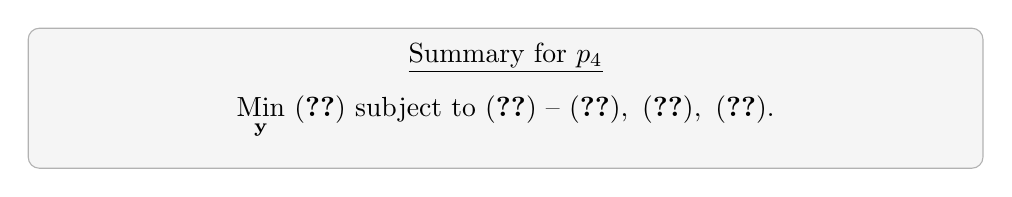
\begin{tikzpicture}
	\node[rectangle, rounded corners, fill=gray!8, draw=gray!60, minimum width=\columnwidth, minimum height=0.7in] at (0,0)(box){};
	\node at (0,0.2in)(title){\underline{Summary for $p_4$}};
	\node at ($(box.south)!0.6!(title.south)$)(text){$
\underset{\mathbf{y}}{\text{Min}} \ \eqref{sec:unconstrainedSchedule:objective} \ \text{subject to} \ \eqref{eqn:obj:power2} \ \text{--} \ \eqref{eqn:objective:energy}, \ \eqref{eqn:defragmentation:active}, \ \eqref{eqn:defragmentation:fragmented}.
$};
\end{tikzpicture}



% imports
\begin{figure*}
\centering
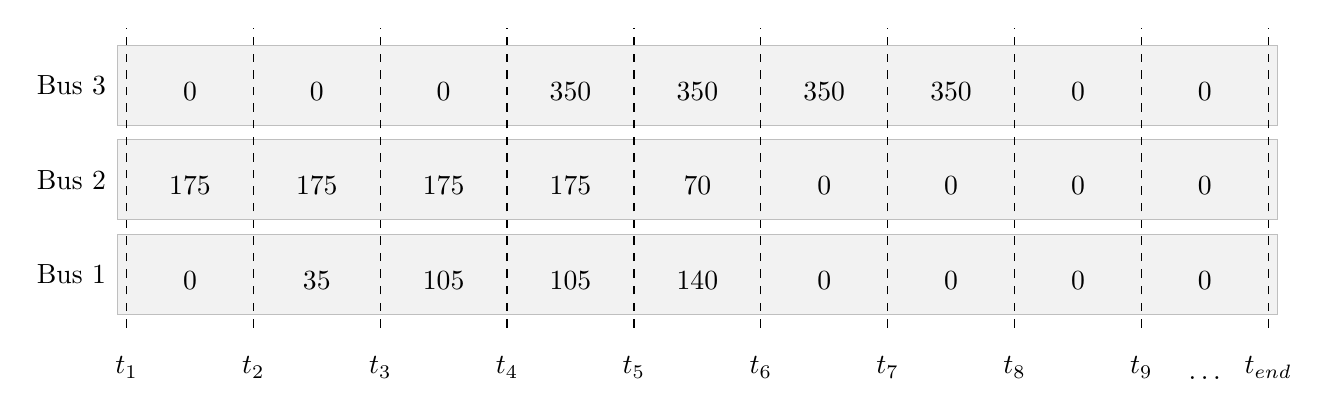
\begin{tikzpicture}
	\node[rectangle, draw=gray!50, fill=gray!10, minimum width=5.8in, minimum height=0.4in](bus1Box) at (7.75,0.8){};
	\node(bus1BoxLabel) at (-0.2, 0.8){Bus 1}; 
	
	\node[rectangle, draw=gray!50, fill=gray!10, minimum width=5.8in, minimum height=0.4in](bus2Box) at (7.75,2){};
	\node(bus1BoxLabel) at (-0.2, 2.0){Bus 2};
	
	\node[rectangle, draw=gray!50, fill=gray!10, minimum width=5.8in, minimum height=0.4in](bus3Box) at (7.75,3.2){};
	\node(bus1BoxLabel) at (-0.2, 3.2){Bus 3};
	
	\foreach \curLab/\preLab[count=\c, evaluate=\c as \pos using {0.5 + (\c - 1)*14.5/9}] in {t_1/t_1, t_2/t_1, t_3/t_2, t_4/t_3, t_5/t_4, t_6/t_7, t_7/t_6, t_8/t_7, t_9/t_8, t_{end}/t_9}
	{
		\node[label=below:$\curLab$](b\c) at (\pos, 0){};
		\node(t) at (\pos, 3.8){};
		\draw[dashed, line width=0.5pt] (b\c.north) -- (t.north); 
		\ifnum\c>1 
			\node(b1Curr) at (\pos, 0.8 - 0.2){};
			\node(b2Curr) at (\pos, 2.0 - 0.2){};
			\node(b3Curr) at (\pos, 3.2 - 0.2){};
			\path(b1Prev.east) -- node(node1\c)[midway, above]{}(b1Curr.west);
			\path(b2Prev.east) -- node(node2\c)[midway, above]{}(b2Curr.west);
			\path(b3Prev.east) -- node(node3\c)[midway, above]{}(b3Curr.west);	
		\fi
			\node(b1Prev) at (\pos, 0.8 - 0.2){};
			\node(b2Prev) at (\pos, 2.0 - 0.2){};
			\node(b3Prev) at (\pos, 3.2 - 0.2){};	
	}
	\path (b9.south) -- node[midway, below=0.1in]{$\hdots$}(b10.south);
	\node at (node12.center){0};
	\node at (node13.center){35};
	\node at (node14.center){105};
	\node at (node15.center){105};
	\node at (node16.center){140};
	\node at (node17.center){0};
	\node at (node18.center){0};
	\node at (node19.center){0};
	\node at (node110.center){0};
	\node at (node22.center){175};
	\node at (node23.center){175};
	\node at (node24.center){175};
	\node at (node25.center){175};
	\node at (node26.center){70};
	\node at (node27.center){0};
	\node at (node28.center){0};
	\node at (node29.center){0};
	\node at (node210.center){0};
	\node at (node32.center){0};
	\node at (node33.center){0};
	\node at (node34.center){0};
	\node at (node35.center){350};
	\node at (node36.center){350};
	\node at (node37.center){350};
	\node at (node38.center){350};
	\node at (node39.center){0};
	\node at (node310.center){0};

\end{tikzpicture}
\caption{An example solution to a 3-bus, 2-charger scenario from the first QP}
\label{fig:solutionExample}
\end{figure*}

\begin{figure*}
\centering
\scalebox{0.8}{
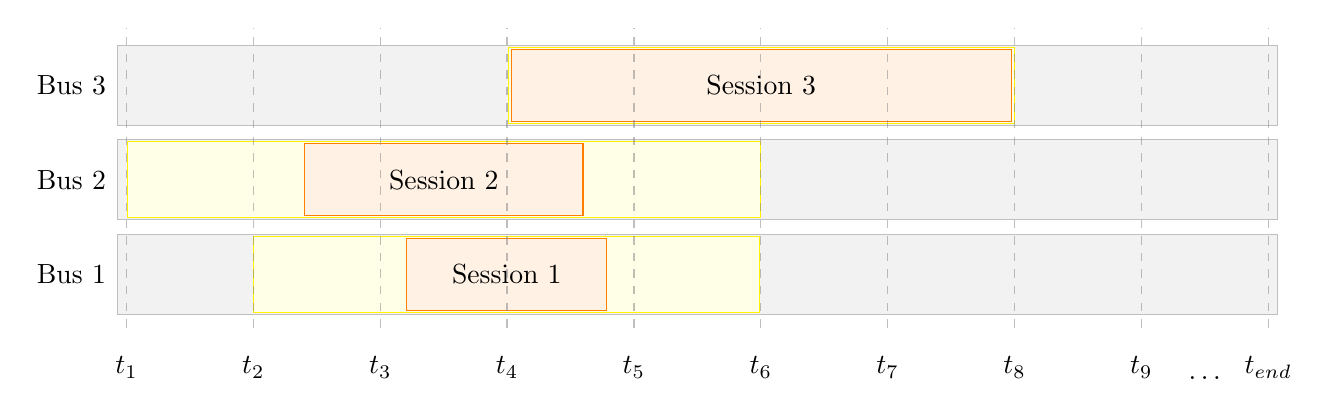
\begin{tikzpicture}
	\node[rectangle, draw=gray!50, fill=gray!10, minimum width=5.8in, minimum height=0.4in](bus1Box) at (7.75,0.8){};
	\node(bus1BoxLabel) at (-0.2, 0.8){Bus 1}; 
	\node[rectangle, draw=yellow!100, fill=yellow!10, minimum width=2.53in, minimum height=0.38in](charge11) at (5.33, 0.8){};
	\node[rectangle, draw=orange!100, fill=orange!10, minimum width=1in, minimum height=0.36in](charge111) at (5.33, 0.8){Session 1};

	\node[rectangle, draw=gray!50, fill=gray!10, minimum width=5.8in, minimum height=0.4in](bus2Box) at (7.75,2){};
	\node(bus1BoxLabel) at (-0.2, 2.0){Bus 2};
	\node[rectangle, draw=yellow!100, fill=yellow!10, minimum width=3.1625in, minimum height=0.38in](charge11) at (4.53, 2){};
	\node[rectangle, draw=orange!100, fill=orange!10, minimum width=1.3915in, minimum height=0.36in](charge111) at (4.53, 2){Session 2};
	
	\node[rectangle, draw=gray!50, fill=gray!10, minimum width=5.8in, minimum height=0.4in](bus3Box) at (7.75,3.2){};
	\node(bus1BoxLabel) at (-0.2, 3.2){Bus 3}; 
	\node[rectangle, draw=yellow!100, fill=yellow!10, minimum width=2.53in, minimum height=0.38in](charge11) at (8.56, 3.2){};
	\node[rectangle, draw=orange!100, fill=orange!10, minimum width=2.50in, minimum height=0.36in](charge111) at (8.56, 3.2){Session 3};


	\foreach \curLab/\preLab[count=\c, evaluate=\c as \pos using {0.5 + (\c - 1)*14.5/9}] in {t_1/t_1, t_2/t_1, t_3/t_2, t_4/t_3, t_5/t_4, t_6/t_7, t_7/t_6, t_8/t_7, t_9/t_8, t_{end}/t_9}
		{
			\node[label=below:$\curLab$](b\c) at (\pos, 0){};
			\node(t) at (\pos, 3.8){};
			\draw[dashed, line width=0.5pt, black!50, opacity=0.5] (b\c.north) -- (t.north); 
		}
		\path (b9.south) -- node[midway, below=0.1in]{$\hdots$}(b10.south); 
\end{tikzpicture}}
\caption{Demonstrates how results from $p_4$ can be reexpressed in terms of continuous variables} 
\label{fig:refactorExample}
\end{figure*}



\begin{figure*}
\centering
\scalebox{0.8}{
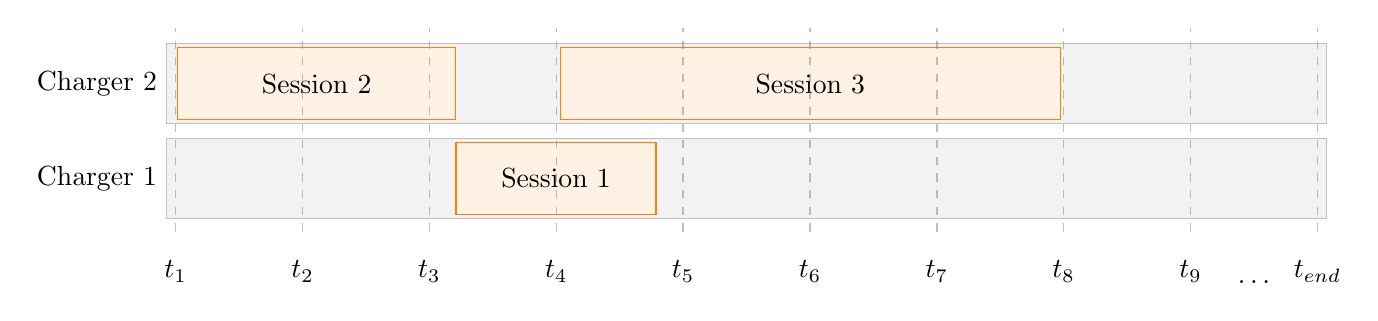
\begin{tikzpicture}
	\node[rectangle, draw=gray!50, fill=gray!10, minimum width=5.8in, minimum height=0.4in](bus1Box) at (7.75,0.8){};
	\node(bus1BoxLabel) at (-0.5, 0.8){Charger 1}; 

	\node[rectangle, draw=gray!50, fill=gray!10, minimum width=5.8in, minimum height=0.4in](bus2Box) at (7.75,2){};
	\node(bus1BoxLabel) at (-0.5, 2.0){Charger 2};
	\node[rectangle, draw=orange!100, fill=orange!10, minimum width=1.3915in, minimum height=0.36in](charge111) at (2.29, 2){Session 2}; 
	\node[rectangle, draw=orange!100, fill=orange!10, minimum width=1in, minimum height=0.36in](charge111) at (5.33, 0.8){Session 1};
	\node[rectangle, draw=orange!100, fill=orange!10, minimum width=2.50in, minimum height=0.36in](charge111) at (8.56, 2){Session 3};


	\foreach \curLab/\preLab[count=\c, evaluate=\c as \pos using {0.5 + (\c - 1)*14.5/9}] in {t_1/t_1, t_2/t_1, t_3/t_2, t_4/t_3, t_5/t_4, t_6/t_7, t_7/t_6, t_8/t_7, t_9/t_8, t_{end}/t_9}
		{
			\node[label=below:$\curLab$](b\c) at (\pos, 0){};
			\node(t) at (\pos, 2.58){};
			\draw[dashed, line width=0.5pt, black!50, opacity=0.5] (b\c.north) -- (t.north); 
		}
		\path (b9.south) -- node[midway, below=0.1in]{$\hdots$}(b10.south); 
\end{tikzpicture}}
\caption{Demonstrates the solution to $p_5$}
\label{fig:secondSolutionExample}
\end{figure*}



\begin{figure*}
\centering
\scalebox{0.8}{
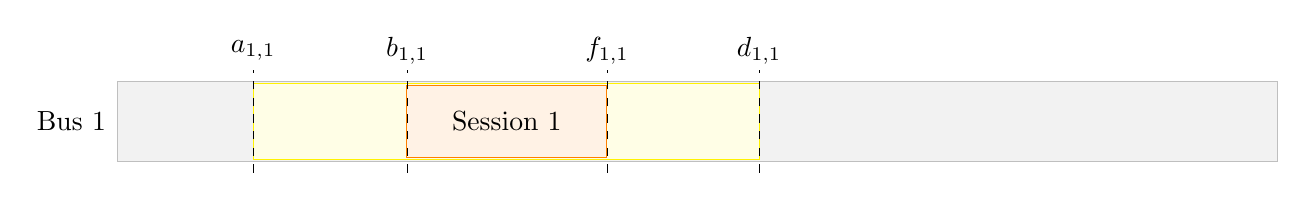
\begin{tikzpicture}
	\node[rectangle, draw=gray!50, fill=gray!10, minimum width=5.8in, minimum height=0.4in](bus1Box) at (7.75,0.8){};
	\node(bus1BoxLabel) at (-0.2, 0.8){Bus 1}; 
	\node[rectangle, draw=yellow!100, fill=yellow!10, minimum width=2.53in, minimum height=0.38in](charge11) at (5.33, 0.8){};
	\node[rectangle, draw=orange!100, fill=orange!10, minimum width=1in, minimum height=0.36in](charge111) at (5.33, 0.8){Session 1}; 
	\draw[dashed] (0.83in,0.15) -- (0.83in,1.45);
	\node at (0.83in,1.7){$a_{1,1}$};
	\draw[dashed] (3.36in, 0.15) -- (3.36in, 1.45);
	\node at (3.36in,1.7){$d_{1,1}$};
	\draw[dashed] (1.6in, 0.15) -- (1.6in, 1.45);
	\node at (1.6in,1.7){$b_{1,1}$};
	\draw[dashed] (2.6in, 0.15) -- (2.6in, 1.45);
	\node at (2.6in,1.7){$f_{1,1}$};
\end{tikzpicture}}
\caption{Gives variables of optimization for $p_5$}
\label{fig:secondProgramVars}
\end{figure*} 


\section{$P_5$: Charger Assignment\label{sec:chargerAssignment}}
The results from $P_4$ give a general estimate of how much and when buses should charge, however we must still address two primary issues. The first is defining concrete start and stop times for each charge session. The second is limiting the charge sessions to a finite number of chargers. 
\par Consider a solution to a three bus, two charger scenario given in Fig.~\ref{fig:solutionExample}.
Note that there appears to be three buses charging at the same time from $t_5$ to $t_6$ even though there are only two chargers.  We can reformulate this solution in terms of continuous start and stop variables and a variable charge rate so that the {\it duration} of each charge session may be relaxed. The objective is to transfer the required energy to the corresponding bus within the optimized charge interval.  
\par Note how few of the charge sessions utilize the chargers to full capacity. This implies that there exists a smaller charge window in which equivalent power can be delivered. This allow us to use the charge durations from the solution from Fig.~\ref{fig:solutionExample} as bounds on {\it allowable} charge windows instead of absolute truth. 
\par An example of how Fig.~\ref{fig:solutionExample} may be reformulated is given in Fig.~\ref{fig:refactorExample}. Note how the actual charge sessions do not necessarily need to take up all the time they were initially allocated in the first solution and that these times can fluctuate if the average charge rate is less than the maximum charger capacity. In this example, we assume a maximum charge capacity of 350kW.  
\par Note how the third charge session does have to be exactly where it was scheduled because the average is equal to the maximum charge rate.
If we examin just the schedule for Bus 1, we note that there are four essential variables for the corresponding charge session: $a(i,r)$, $b(i,r)$, $f(i,r)$ and $d(i,r)$ which represent the minimum start time, actual start time, actual end time, and maximum end time, respectively. 
\par The problem we must now solve is one of arranging these intervals such that each one is larger than its minimum width (or charge time).  We must also account for the number of chargers. It can be helpful to view the problem as a bin packing problem, where each session must fit within the ``swim lane'' of a charger.  For example, taking the charge sessions given in Fig.~\ref{fig:refactorExample} and arranging them so that there is no overlap between sessions will yield a valid solution as shown in Fig.~\ref{fig:secondSolutionExample}.
From Fig.~\ref{fig:secondProgramVars}, we know that $a(i,r), b(i,r),f(i,r)$ and $d(i,r)$ must be such that 
\begin{equation}\label{eqn:assignment:eqn1}
%\begin{aligned}
	a(i,r) \leq b(i,r) \leq f(i,r) \leq d(i,r),
	%a(i,r) \le b(i,r) \\
	%b(i,r) \le f(i,r) \\
	%f(i,r) \le d(i,r). 	
%\end{aligned}
\end{equation}
where $a(i,r)$ and $d(i,r)$ are known from $P_4$, and $b(i,r)$ and $f(i,r)$ are optimization variables. 
\par To differentiate between different chargers, define $\sigma(i,r,k)$ as a binary selector variable which is one if charger $k$ services bus $i$ for session $r$ and zero otherwise. Because only one charger can charge each bus at a time and each charge session {\it must} be serviced, we have
\begin{equation}\label{eqn:assignment:eqn2}
	\sum_k \sigma(i,r,k) = 1  \ \forall i,r.
\end{equation}
\par Next, we also know that during each session a certain amount of energy must be transfered from the charger to the battery.  The amount of energy that must be transfered to bus $i$ during session $r$ is given in the solution to $P_4$ and are denoted $e(i,r)$. We can compute a minimum time window from these values by letting 
\begin{equation}\label{eqn:assignment:eqn3}
	w(i,r)_{\text{min}} = \frac{e(i,r)}{p_\text{max}}.
\end{equation}
If we include constraints for a minimum time per session, then the previous expression becomes
\begin{equation*}
	w(i,r)_{\text{min}} = \text{max}\left ( w_{\text{min}}, \frac{e(i,r)}{p_\text{max}} \right )
\end{equation*}
Because this is the minimum time window, we must ensure that the difference between the start and stop times is at least this large so that
\begin{equation}\label{eqn:assignment:eqn4}
	f(i,r) - b(i,r) \ge w(i,r) \ \forall i,r.
\end{equation}
\par The final set of constraints deals with contention so that no charger can be scheduled for two sessions that overlap. Let $\mathcal{L} = \{(i,r)\times (i',r') \}$ where charge sessions $i,r$ and $i',r'$ have the potential to overlap. Before we can prevent overlap, we must define a binary variable $l(i,r,i',r')$ which is equal to one when session $i,r$ is scheduled before session $i',r'$ and zero otherwise so that
\begin{equation}
	\begin{cases}
		f(i,r) \le b(i',r') & l(i,r,i',r') = 1 \\
		f(i',r') \le b(i',r') & l(i,r,i',r') = 0 
	\end{cases}
\end{equation}
To simplify these constraints, let $M$ have a large value such as the number of seconds in a day. We know what the top constraint must be trivially satisfied when $l(i,r,i',r') = 0$ and the bottom must also when $l(i,r,i',r') = 1$.  This leads to a reformulation so that
\begin{equation*}\begin{aligned}
		f(i,r) - b(i',r') & \le M(1 - l(i,r,i',r')\\
		f(i',r') - b(i,r) & \le l(i,r,i',r')M  
\end{aligned}\end{equation*}
However, this constraint {\it only} needs to hold when sessions $i,r$ and $i',r'$ are scheduled to charge on the same charger or that $\sigma(i,r,k) = \sigma(i',r',k) = 1$. We can reformulate the above constraint to satisfy this condition by letting
\begin{equation}\label{eqn:assignment:eqn5}\begin{aligned}
	f(i,r) - b(i',r') & \le M(3 - \sigma(i,r,k) - \sigma(i',r',k) - l(i,r,i',r')) \\
	f(i',r') - b(i,r) & \le M(2 - \sigma(i,r,k) - \sigma(i',r',k) + l(i,r,i',r'))
\end{aligned}\end{equation}
\par Finally, we desire the schedule to closly match the charge plan from $P_4$, which occures when each charge session matches the durations given in $P_4$ and so we formulated an objective function which minimizes the differences in the given plan and the results from $P_4$ by letting the objective be
\begin{equation}\label{eqn:assignment:eqn6}
	\underset{f,b}{\text{min}} \sum_{i,r}\lVert b(i,r) - a(i,r)\rVert_2^2 + \lVert f(i,r) - d(i,r) \rVert_2^2
\end{equation}
which has the effect of driving each variable to the desired value and more heavily penalizing values that are further from their optimal.
The final optimization problem is given below.\\[0.1in]
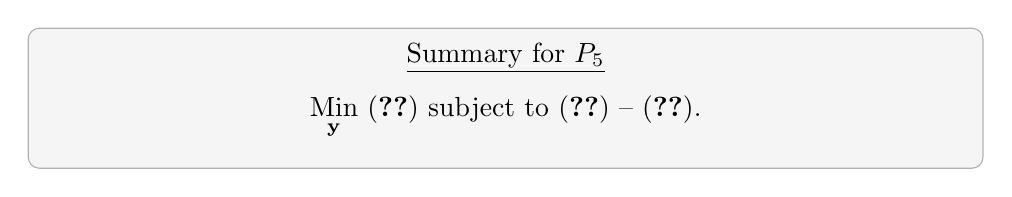
\begin{tikzpicture}
	\node[rectangle, rounded corners, fill=gray!8, draw=gray!60, minimum width=\columnwidth, minimum height=0.7in] at (0,0)(box){};
	\node at (0,0.2in)(title){\underline{Summary for $P_5$}};
	\node at ($(box.south)!0.6!(title.south)$)(text){$
	\underset{\mathbf{y}}{\text{Min}} \ \eqref{eqn:assignment:eqn6} \ \text{subject to} \ \eqref{eqn:assignment:eqn1} \ \text{--} \ \eqref{eqn:assignment:eqn5}.
$};
\end{tikzpicture}
\par Ideally, when $P_5$ is solved to optimality, the chargers are fully utilized. However, optimality for $P_5$ is computationally demanding and scalable solutions may require relaxations in the optimality gap.  However, increasing the gap leads to a solution in which chargers are not fully utilized. The next section uses the session ordering from $P_5$, but recomputes session start/stop times to better utilize the charger availability even when sub-optimal gaps are given for $P_5$.


\section{$P_6$: Optimizing Charge Schedules\label{sec:optimizingChargeSchedules}}
Many times it is not feasible to compute the optimal set of charge schedules given in the previous sections. As the number of buses and charge sessions becomes large, computing a small-gap solution becomes computationally untractable. Allowing solutions with larger optimality gaps decreases the number of computations, but results in sub-optimal charge-time windows.  In this section, a more optimal set of charge windows is computed using the results from $P_5$ to infer charger assignment and ordering for each charge session. We also know that the optimal solution will expand the charge windows to use any available time where a charger is unused, implying that the ``stop'' time for each session will either be equal to its buse's departure time, or the start time of the next window which can be expressed as
\begin{equation}\label{eqn:optChargeSchedules:eqn1}
\begin{cases}
	c(s,i,r+1) = c(f,i,r) & c(d,i,r) > c(a,i,r+1)\\[0.08in]
	\begin{aligned}
	c(s,i,r+1) &= c(a,i,r+1) \\
	c(f,i,r) &= c(d,i,r)
	\end{aligned} & c(d,i,r) <= c(a,i,r+1) \\
\end{cases}
\end{equation}
where $c(s,i,r)$ is the start time for charger $i$'s $r^{\text{th}}$ charge session, $c(f,i,r)$ is the stop time for charger $i$'s $r^{\text{th}}$ charge session, $c(d,i,r)$ is the departure time for the bus scheduled for charger $i$'s $r^{\text{th}}$ charge session, and $c(a,i,r)$ is the arrival time for the bus scheduled for charger $i$'s $r^{\text{th}}$ charge session. 
The minimum charge length must also be used so that energy can be properly delivered, so that
\begin{equation}\label{eqn:optChargeSchedules:eqn2}
	c(f,i,r) - c(s,i,r) \ge w(i,r)
\end{equation}
where $w(i,r)$ is the minimum charge time for the corresponding session.
\par The final step to optimizing the charge windows is to give preference to windows with larger power deliveries. Let the objective for the optimization program be 
\begin{equation}\label{eqn:optChargeSchedule:objective}
	J_{\text{window}} = \frac{1}{n}\sum_{i,r} \left \lVert \frac{c(f,i,r) - c(s,i,r)}{e(i,r)} \right \rVert^2_2.
\end{equation}
When the function $J$ contains windows with equal amounts of energy, the minimum will be found where each charge interval is the same width. As the amount of energy increases, the objective penalizes less for larger window sizes and thus gives preference to high energy sessions.
The final optimization problem is given below.\\[0.1in]
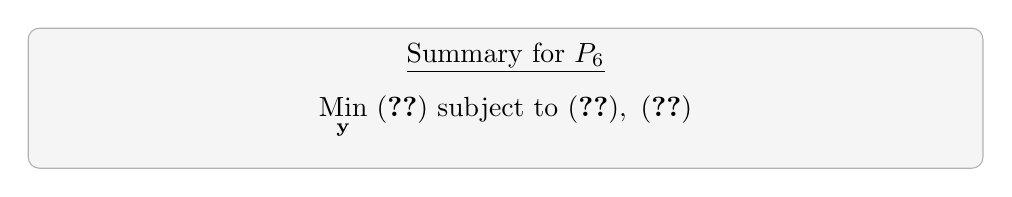
\begin{tikzpicture}
	\node[rectangle, rounded corners, fill=gray!8, draw=gray!60, minimum width=\columnwidth, minimum height=0.7in] at (0,0)(box){};
	\node at (0,0.2in)(title){\underline{Summary for $P_6$}};
	\node at ($(box.south)!0.6!(title.south)$)(text){$ 
	\underset{\mathbf{y}}{\text{Min}} \ \eqref{eqn:optChargeSchedule:objective} \ \text{subject to} \ \eqref{eqn:optChargeSchedules:eqn1}, \ \eqref{eqn:optChargeSchedules:eqn2}
$};
\end{tikzpicture} 
\par After solving $P_6$ each charge session is assigned to a charger so that contention for limited chargers has been managed for each group. Furthermore, each session also specifies target energy requirements which manage the risks of depleting batteries but does not give instructions on how the energy is to be delivered. The energy delivery problem is addressed in the next section and combined results for all groups so that the charge schedule begins to approach a globally optimal solution.

\section{$p_7:$ Constrained Schedule\label{sec:constrainedSchedule}}
Up to this point, we have computed the ``optimal'' schedule which assumes any bus can charge without regard to the number of chargers. We then separate buses into groups to reduce the scope of the problem and treat each sub-problem separately while we defragment and assign each charge session to specific chargers before determining the final start and stop times for each bus's charge session.
\par The final step in this process is to determine how the energy will be delivered so that cost is minimised. Begin with constraints for bus power, energy, and cost from Section \ref{sec:unconstrainedSchedule} that are given in \eqref{eqn:obj:power2}, \eqref{eqn:battery:busPower}, \eqref{eqn:objective:pt}, \eqref{eqn:objective:p15}, \eqref{eqn:objective:pFac}, \eqref{eqn:objective:pDem} and \eqref{eqn:objective:energy}. Next, include constraints for energy so that the energy for each charge session is properly delivered using a modified version of Eqn. \eqref{eqn:defragmentation:active} so that
\begin{equation}\label{eqn:constrainedSchedule:modified}
	\mathbf{b}(i,:)\rho(i,r) = \psi(i,r),
\end{equation}
where $\psi(i,r)$ is the required energy for bus $i$ during rest period $r$ as computed from the solution of the De-Fragmentation problem.
\\[0.1in] 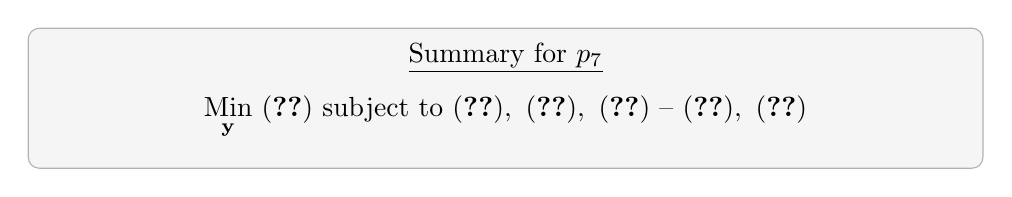
\begin{tikzpicture}
	\node[rectangle, rounded corners, fill=gray!8, draw=gray!60, minimum width=\columnwidth, minimum height=0.7in] at (0,0)(box){};
	\node at (0,0.2in)(title){\underline{Summary for $p_7$}};
	\node at ($(box.south)!0.6!(title.south)$)(text){$
	\underset{\mathbf{y}}{\text{Min}} \ \eqref{sec:unconstrainedSchedule:objective} \ \text{subject to} \ \eqref{eqn:obj:power2}, \ \eqref{eqn:battery:busPower}, \ \eqref{eqn:objective:pt} \ \text{--} \ \eqref{eqn:objective:energy}, \ \eqref{eqn:constrainedSchedule:modified}
$};
\end{tikzpicture}
\section{$p_8:$ Constrained Smooth Schedule\label{sec:constrainedSmoothSchedule}}
 \par The charge schedule from $p_7$ will contain the same on-off defects as the solution to $p_1$ which can be managed as before by executing $p_7$ once again with two changes: The first constrains the objective so that it achieves the optimal cost. The second reduces the difference of adjacent charge rates with the smoothing objective from \eqref{eqn:objective:smooth}.
\\[0.1in] 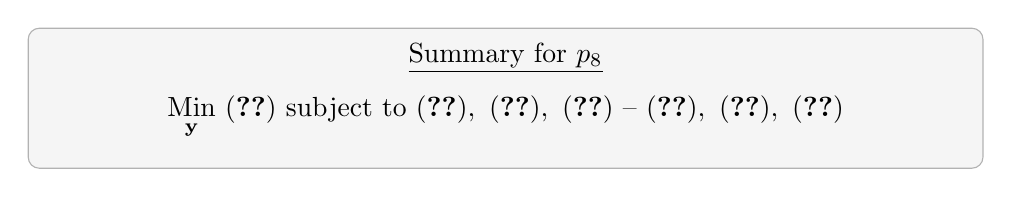
\begin{tikzpicture}
	\node[rectangle, rounded corners, fill=gray!8, draw=gray!60, minimum width=\columnwidth, minimum height=0.7in] at (0,0)(box){};
	\node at (0,0.2in)(title){\underline{Summary for $p_8$}};
	\node at ($(box.south)!0.6!(title.south)$)(text){$
	\underset{\mathbf{y}}{\text{Min}} \ \eqref{eqn:objective:smooth} \ \text{subject to} \ \eqref{eqn:obj:power2}, \ \eqref{eqn:battery:busPower}, \ \eqref{eqn:objective:pt} \ \text{--} \ \eqref{eqn:objective:energy}, \ \eqref{eqn:unconstrainedSmooth:equivalence}, \ \eqref{eqn:constrainedSchedule:modified}
$};
\end{tikzpicture}


\section{Results}
-- describe pro-time vs pro-route scenarios
-- describe battery capacities
-- describe maximum charge rates
-- describe how route scheduels, delta, and uncontrolled loads come from uta.
-- describe the gaps used in the minimisation algorithms.
\subsection{Comparison with Prior Work}
In this section, we compare the proposed method with a baseline algorithm and a method developed be \textcolor{red}{insert reference to He. et al here}. The baseline method models how bus drivers charge their electric vehicles at the Utah Transit Authority in Salt Lake City, Utah. At UTA, when bus drivers arrive at the station, they refuel their electric buses whenever a charger is available so that the number of charge sessions is maximized. The method from \textcolor{red}{He et al.} works somewhat differently by minimising the cost of energy with respect to the time of use tarrifs $\mu_{e-on}$ and $\mu_{e-off}$.
\par The comparison we observe is given for a 5-bus, 5-charger scenario with a pro-time preference and a single group. Each method was run, and the cost related to demand, facilities, and energy charges are given in Fig. \ref{fig:results:costComparison}. Note how the baseline algorithm suffers significantly from the demand charges associated with On-Peak Power, and \textcolor{red}{He et al.} incurres additional cost from the facilities charges, indicating that an emphasis on energy charges and habitual charging patterns can be improved.
\par We observe where the differences in cost originate in Fig. \ref{fig:results:totalPower}. Observe how the baseline charge profile achieved the largest 15-minute average power between 19:12 adn 21:36 which is during on-peak hours and consequently yielded the large On-Peak Power charges given in Fig. \ref{fig:results:costComparison}. Additionally, note how the proposed method maintains a relatively flat power profile so that the load is balanced throughout the day which we investigate in Fig. \ref{fig:results:powerPlot}.
\par We investigate how t 
\begin{figure}
	\centering
	\makeComparisonBarChartThree{media/11_results/costComparison.csv}{Cost (Dollars)}{Baseline}{He et al.}{Proposed}
	\caption{Cost comparison with prior work}
	\label{fig:results:costComparison}
\end{figure} 

 
\begin{figure*}
	\centering
	\makeComparisonPower{media/11_results/powerPlotfiscal.csv}{media/11_results/powerPlotconsumption.csv}{15-Minute Average Power (kW)}{Proposed}{He et al.}
	\caption{Comparison between uncontrolled and bus loads}
	\label{fig:results:powerPlot}
\end{figure*}


\begin{figure*}
	\centering
	\makeComparisonTotalPower{media/11_results/totalPowerfiscalproTime.csv}{media/11_results/totalPowerconsumptionproTime.csv}{15-Minute Average Power (kW)}{Proposed}{He et al.}
	\caption{15-Minute average power for one day}
	\label{fig:results:totalPower}
\end{figure*}



\subsection{Contention: Sub-Optimal Schedules}
show comparison of schedules with large vs small gaps when finding charge schedules. Talk about how the computation time significantly increases as the gap decreases. Show that a smaller gap may be desireable as this lengthens charge times so that they are easier to implement in reality. Explain that we trade time for longer charge sessions better suited for operations.
\input{media/11_results/disoptimalRoutes.tex}
\input{media/11_results/sessionImageStyle}
\begin{figure*}
\begin{tikzpicture}
\begin{axis}[colorbar, ChargeSessionImage, width=0.95\textwidth, height=0.5\textwidth, point meta min=0, point meta max=350, xmin=0.5, xmax=4320.5,xtick={540, 1080, 1620, 2160, 2700, 3240, 3780, 4320}, xticklabels={3:00, 6:00, 9:00, 12:00, 15:00, 18:00, 21:00, 0:00}, ymin=0.5, ymax=18.5]

\addplot [forget plot] graphics [xmin=0.5, xmax=4320.5, ymin=0.5, ymax=18.5] {media/11_results/optimalRoutes-1.png};
\end{axis}

\end{tikzpicture}%
\caption{Routes with a small gap in the route placement problem}
\label{fig:results:optimalRoutes}
\end{figure*}


\subsection{Contested vs Uncontested}
address that there is significantly more computations for the schedules that are operations-oriented, and use this to segway into groups
\begin{figure}
	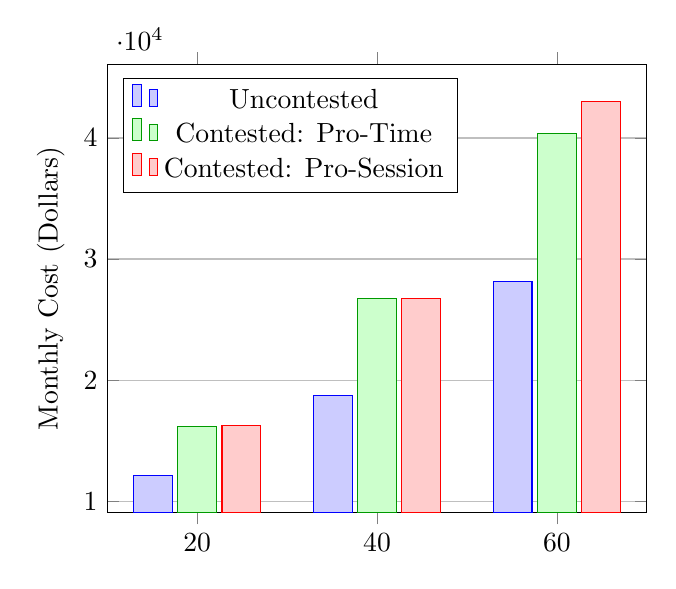
\begin{tikzpicture}
		\begin{axis}[ybar, bar width=14pt, xmin=10, xmax=70, xtick={20, 40, 60},ymajorgrids=true, ylabel={Monthly Cost (Dollars)}, legend pos=north west]
			\addplot[fill=blue!20, draw=blue] coordinates {
				(20, 12150.65)
				(40, 18745.58)
				(60, 28166.09)
			};
			\addplot[fill=green!20, draw=black!40!green] coordinates {
				(20, 16183.79)
				(40, 26738.71)
				(60, 40405.72)
			};
			\addplot[fill=red!20, draw=red] coordinates {
				(20, 16256.21)
				(40, 26738.71)
				(60, 43007.78)
			};
		\legend{Uncontested, Contested: Pro-Time, Contested: Pro-Session};
		\end{axis}
	\end{tikzpicture}
	\caption{Comparison of Monthly Costs}
	\label{fig:results:contestedVsUncontestedPrice}
\end{figure}



\begin{figure}\centering
	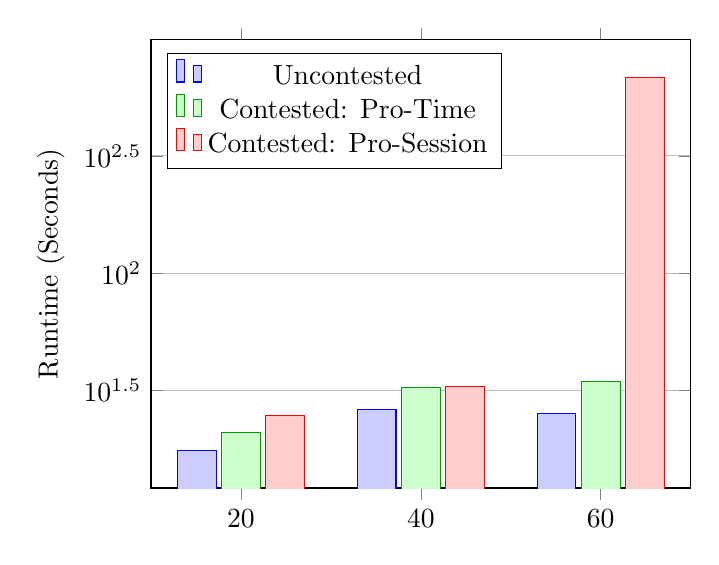
\begin{tikzpicture}
		\begin{axis}[ybar, bar width=14pt, xmin=10, xmax=70, xtick={20, 40, 60},ymajorgrids=true, ylabel={Runtime (Seconds)}, ymode=log, legend pos=north west]
			\addplot[fill=blue!20, draw=blue] coordinates {
				(20, 17.46)
				(40, 26.09)
				(60, 25.17)
			};
			\addplot[fill=green!20, draw=black!40!green] coordinates {
				(20, 20.84)
				(40, 32.47)
				(60, 34.46)
			};
			\addplot[fill=red!20, draw=red] coordinates {
				(20, 24.57)
				(40, 32.70)
				(60, 686.40)
			};
		\legend{Uncontested, Contested: Pro-Time, Contested: Pro-Session};
		\end{axis}
	\end{tikzpicture}
	\caption{Comparison of Runtimes} 
	\label{fig:results:contestedVsUncontestedTime}
\end{figure}



%\begin{figure}
	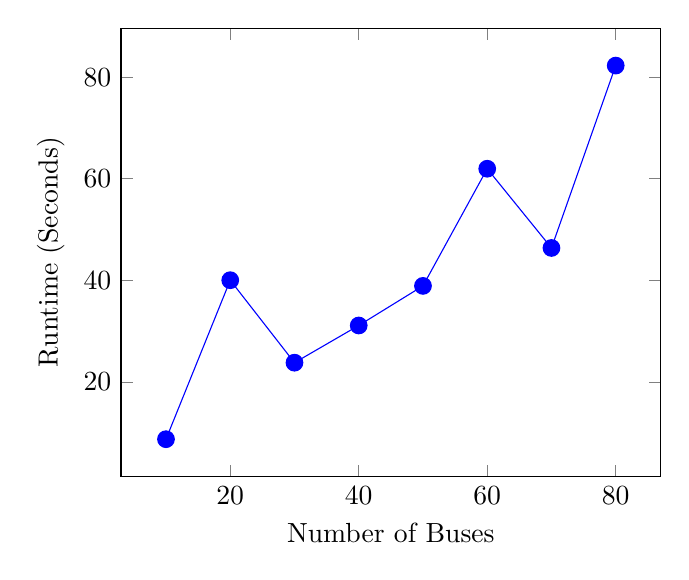
\begin{tikzpicture}
		\begin{axis}[xlabel=Number of Buses,  ylabel=Runtime (Seconds)]
			\addplot[blue] coordinates {
				(10, 8.69)
				(20, 40.01)
				(30, 23.76)
				(40, 31.09)
				(50, 38.89)
				(60, 61.97)
			  (70, 46.36 )
			  (80, 82.29)};
			\addplot[blue, only marks, mark size=3pt] coordinates {
			  (10, 8.69)
				(20, 40.01)
				(30, 23.76)
				(40, 31.09)
				(50, 38.89)
				(60, 61.97)
			  (70, 46.36 )
			  (80, 82.29)};
		\end{axis}
	\end{tikzpicture}
	\caption{Uncontested Runtime} 
	\label{fig:uncontestedRuntime}
\end{figure}



%\begin{figure}
	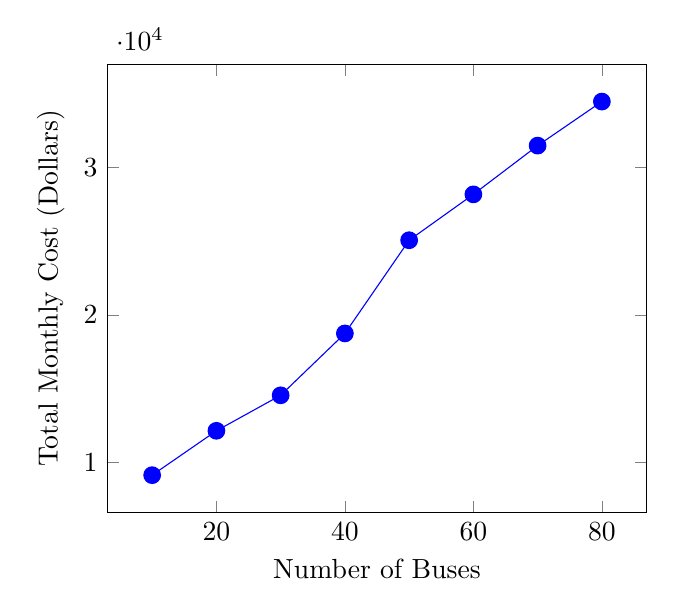
\begin{tikzpicture}
		\begin{axis}[xlabel=Number of Buses, ylabel=Total Monthly Cost (Dollars), legend pos=north west, legend style={nodes={scale=0.7}}]
			\addplot[blue] coordinates {
				(10,  9145.28)
				(20, 12150.65)
				(30, 14554.62)
				(40, 18745.58)
				(50, 25059.45)
				(60, 28166.09)
				(70, 31468.65)
				(80, 34452.85)}; 
			\addplot[blue, only marks, mark size=3pt] coordinates {
				(10,  9145.28)
				(20, 12150.65)
				(30, 14554.62)
				(40, 18745.58)
				(50, 25059.45)
				(60, 28166.09)
				(70, 31468.65)
				(80, 34452.85)}; 
			%\legend{Proposed, Baseline, He et al.}
		\end{axis}
	\end{tikzpicture}
	\caption{Monthly Cost With Contention with emphasis on time}
	\label{fig:scalabilityCostContentionProTime}
\end{figure}



%\begin{figure}
	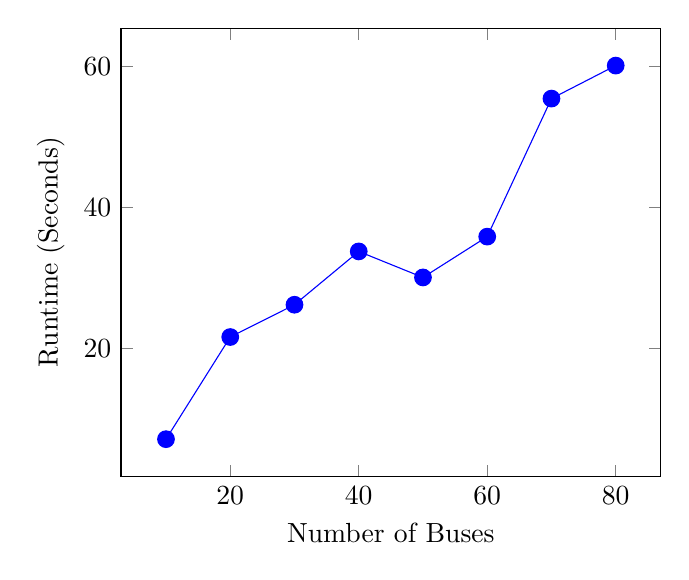
\begin{tikzpicture}
		\begin{axis}[xlabel=Number of Buses,  ylabel=Runtime (Seconds)]
			\addplot[blue] coordinates {
				(10, 7.15)
				(20, 21.64)
				(30, 26.22)
				(40, 33.78)
				(50, 30.09)
				(60, 35.88)
			  (70, 55.46 )
			  (80, 60.14)};
			\addplot[blue, only marks, mark size=3pt] coordinates {
				(10, 7.15)
				(20, 21.64)
				(30, 26.22)
				(40, 33.78)
				(50, 30.09)
				(60, 35.88)
			  (70, 55.46 )
			  (80, 60.14)};
		\end{axis}
	\end{tikzpicture}
	\caption{Runtime with contention with time prioritized} 
	\label{fig:uncontestedRuntime}
\end{figure}




\subsection{Contention: The Importance of Groups}
Show time difference between 1, 2, and 3 groups when optimizing for cost, talk about how this disparity significantly increases as the gap requirements decrease.
\begin{figure}
\centering
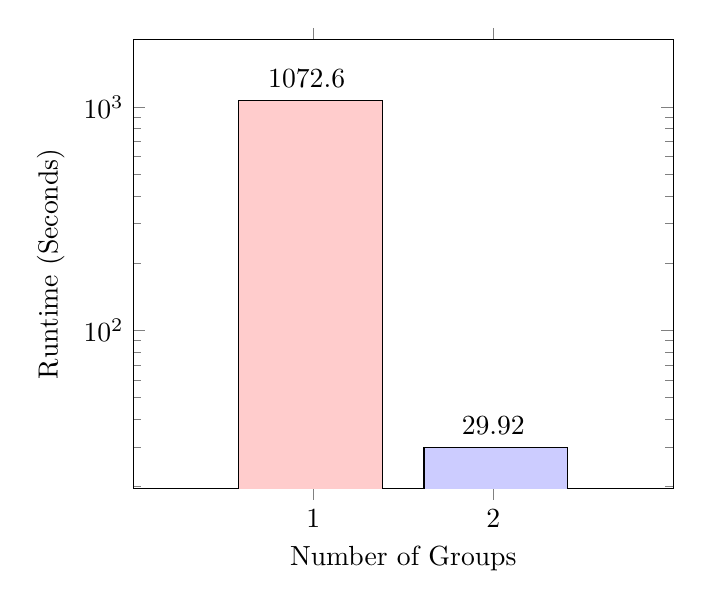
\begin{tikzpicture}
	\begin{axis}[ybar, ymode=log, ymax=2000, xmin=0, xmax=3, xtick={1,2}, xlabel=Number of Groups, ylabel=Runtime (Seconds)]
		\addplot[fill=red!20, bar width=0.8] coordinates {(1.4, 1072.6)};
		\addplot[fill=blue!20, bar width=0.8]  coordinates {(1.6, 29.92)};
	\end{axis}
	\node at (2.2,5.2){1072.6};
	\node at (4.57, 0.79){29.92};
\end{tikzpicture}
\caption{Runtimes for a 18 bus 12 charger scenario at a 0.13\% gap}
\label{fig:results:groupResults}
\end{figure}

\subsection{Effecrts of De-Fragmentation}
display heat map of before and after for contested case.
\begin{figure*}
\centering
\begin{tikzpicture} 
\begin{axis}[colorbar, ChargeSessionImage, width=5.2in, height=2in, point meta min=0, point meta max=350, xmin=0.5, xmax=4320.5, xtick={540, 1080, 1620, 2160, 2700, 3240, 3780, 4320}, xticklabels={3:00, 6:00, 9:00, 12:00, 15:00, 18:00, 21:00, 0:00}, ymin=0.5, ymax=40.5]
\addplot [forget plot] graphics [xmin=0.5, xmax=4320.5, ymin=0.5, ymax=40.5] {\rootdirectorythree/media/11_results/defragmentedChargeLimit-1.png}; 
\end{axis} 
\end{tikzpicture}
\caption{Routes with De-Fragmentation}
\label{fig:results:defragmentedChargeLimit}
\end{figure*}

\begin{figure*}
\centering
\begin{tikzpicture} 
\begin{axis}[colorbar, ChargeSessionImage, width=0.95\textwidth, height=0.5\textwidth, point meta min=0, point meta max=350, xmin=0.5, xmax=4320.5, xtick={540, 1080, 1620, 2160, 2700, 3240, 3780, 4320}, xticklabels={3:00, 6:00, 9:00, 12:00, 15:00, 18:00, 21:00, 0:00}, ymin=0.5, ymax=40.5]
\addplot [forget plot] graphics [xmin=0.5, xmax=4320.5, ymin=0.5, ymax=40.5] {media/11_results/noFragmentationChargeLimit-1.png}; 
\end{axis} 
\end{tikzpicture}
\caption{Routes without De-Fragmentation}
\label{fig:results:noFragmentationChargeLimit}
\end{figure*}


describe how defragmentation affects runtime and cost in the case of time-oriented and operations-oriented approaches.
\begin{figure}\centering
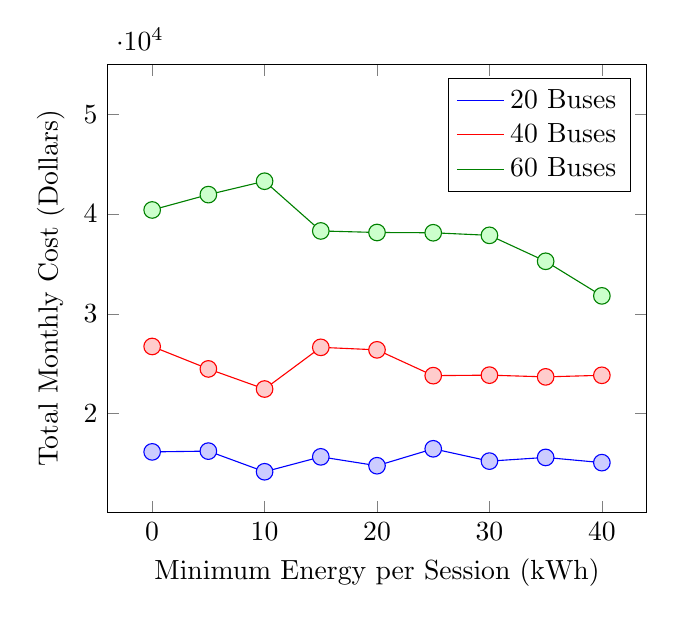
\begin{tikzpicture}
\begin{axis}[xlabel=Minimum Energy per Session (kWh), ylabel=Total Monthly Cost (Dollars), ymax=55000, legend pos=north east]
	\addplot[blue] coordinates {
		(0, 16183.79)   
	  (5, 16260.98)  
		(10,14194.10)  
		(15,15686.16)  
		(20,14798.53)  
		(25,16492.56)  
		(30,15259.19)  
		(35,15628.38)  
		(40,15106.82)};
\addplot[red] coordinates {
		(0, 26738.71)
		(5, 24491.03)
	  (10,22476.88)
		(15,26650.71)
		(20,26400.31)
		(25,23816.91)
		(30,23866.55)
		(35,23693.25)
		(40,23851.78)};
\addplot[green!50!black] coordinates {
		(0, 40405.72)
		(5, 41942.45)
	  (10,43284.09)
		(15,38304.96)
		(20,38150.28)
		(25,38122.51)
		(30,37864.79)
		(35,35268.11)
		(40,31805.12)};

\addplot[blue!20, draw=blue, only marks, mark size=3pt] coordinates {
		(0, 16183.79)  
		(5, 16260.98)  
	  (10,14194.10)  
		(15,15686.16)  
		(20,14798.53)  
		(25,16492.56)  
		(30,15259.19)  
		(35,15628.38)   
		(40,15106.82)};
\addplot[red!20, draw=red, only marks, mark size=3pt] coordinates {
	(0, 26738.71)  	
	(5, 24491.03)  	
	(10,22476.88)   
	(15,26650.71)  	
	(20,26400.31)  	
	(25,23816.91)  	
	(30,23866.55)  	
	(35,23693.25)  	
	(40,23851.78)};	
\addplot[green!20, draw=green!50!black, only marks, mark size=3pt] coordinates {
	(0, 40405.72)  
	(5, 41942.45)  
	(10,43284.09)  
	(15,38304.96)  
	(20,38150.28)  
	(25,38122.51)  
	(30,37864.79)  
	(35,35268.11)  
	(40,31805.12)};

\legend{20 Buses, 40 Buses, 60 Buses} 
\end{axis}
\end{tikzpicture}
\caption{Cost comparison of different degragmentation thresholds in a pro-time optimization scheme.}
\label{fig:results:defragmentationCostProTime}
\end{figure}

\begin{figure}
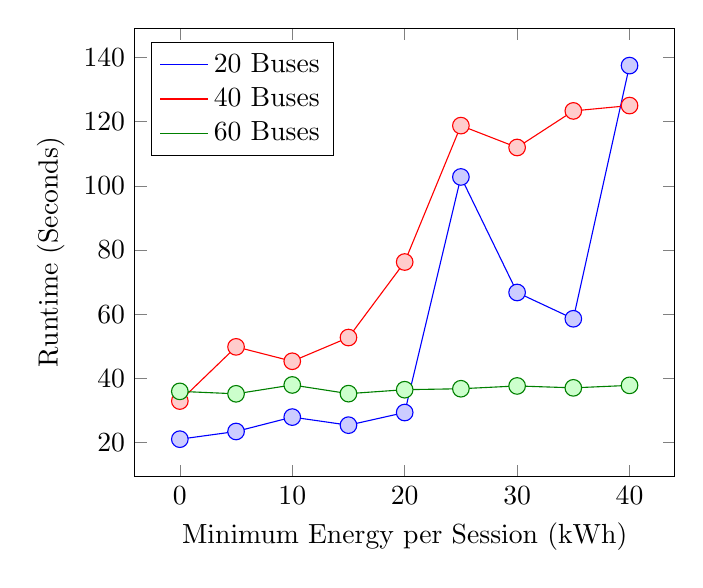
\begin{tikzpicture}
\begin{axis}[xlabel=Minimum Energy per Session (kWh), ylabel=Runtime (Seconds), legend pos=north west]
	\addplot[blue] coordinates {
		(0, 21.00)
		(5, 23.40)
	  (10,27.89)
		(15,25.37)
		(20,29.31)
		(25,102.78)
		(30,66.75)
		(35,58.55)
		(40,137.51)}; 
\addplot[red] coordinates {
		(0, 32.89)
		(5, 49.79)
	  (10,45.30)
		(15,52.70)
		(20,76.25)
		(25,118.79)
		(30,111.97)
		(35,123.37)
		(40,125.04)}; 
\addplot[green!50!black] coordinates {
		(0, 35.91)
		(5, 35.15)
	  (10,37.91)
		(15,35.20)
		(20,36.43)
		(25,36.73)
		(30,37.60)
		(35,37.01)
		(40,37.78)}; 
\addplot[blue!20, draw=blue, only marks, mark size=3pt] coordinates {
		(0, 21.00)
		(5, 23.40)
	  (10,27.89)
		(15,25.37)
		(20,29.31)
		(25,102.78)
		(30,66.75)
		(35,58.55)
		(40,137.51)}; 
\addplot[red!20, draw=red, only marks, mark size=3pt] coordinates {
		(0, 32.89)
		(5, 49.79)
	  (10,45.30)
		(15,52.70)
		(20,76.25)
		(25,118.79)
		(30,111.97)
		(35,123.37)
		(40,125.04)}; 
\addplot[green!20, draw=green!50!black, only marks, mark size=3pt] coordinates {
		(0, 35.91)
		(5, 35.15)
	  (10,37.91)
		(15,35.20)
		(20,36.43)
		(25,36.73)
		(30,37.60)
		(35,37.01)
		(40,37.78)}; 
\legend{20 Buses, 40 Buses, 60 Buses}		
\end{axis}
\end{tikzpicture}
\caption{Comparison of runtime for the uncontested and contested scenarios over different de-fragmentation criteria}
\label{fig:results:runtimeDefragmentation}
\end{figure}

\begin{figure}
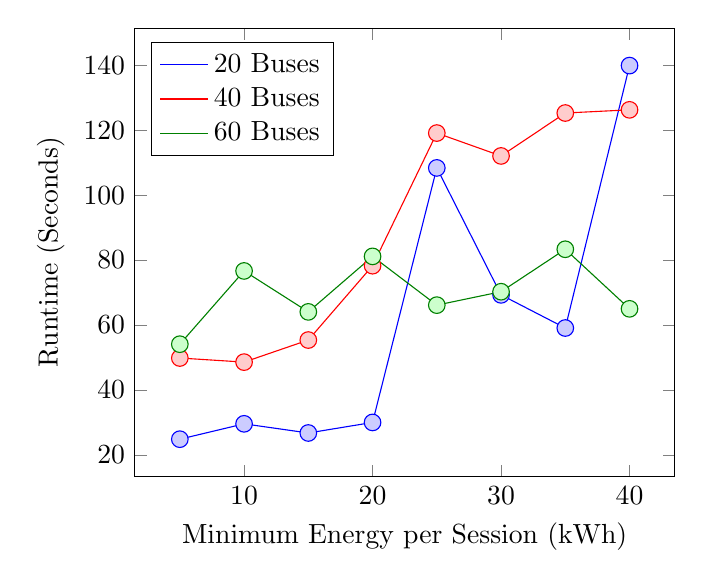
\begin{tikzpicture}
\begin{axis}[xlabel=Minimum Energy per Session (kWh), ylabel=Runtime (Seconds), legend pos=north west]
	\addplot[blue] coordinates {
		(5, 24.83)
	  (10,29.56)
		(15,26.74)
		(20,29.99)
		(25,108.38)
		(30,69.28)
		(35,59.07)
		(40,139.90)}; 
\addplot[red] coordinates {
		(5, 49.83)
	  (10,48.57)
		(15,55.37)
		(20,78.26)
		(25,119.12)
		(30,112.07)
		(35,125.29)
		(40,126.27)}; 
\addplot[green!50!black] coordinates {
		(5, 54.09)
	  (10,76.65)
		(15,64.04)
		(20,81.13)
		(25,66.12)
		(30,70.25)
		(35,83.33)
		(40,64.98)}; 
\addplot[blue!20, draw=blue, only marks, mark size=3pt] coordinates {
		(5, 24.83)
	  (10,29.56)
		(15,26.74)
		(20,29.99)
		(25,108.38)
		(30,69.28)
		(35,59.07)
		(40,139.90)}; 
\addplot[red!20, draw=red, only marks, mark size=3pt] coordinates {
		(5, 49.83)
	  (10,48.57)
		(15,55.37)
		(20,78.26)
		(25,119.12)
		(30,112.07)
		(35,125.29)
		(40,126.27)}; 
\addplot[green!20, draw=green!50!black, only marks, mark size=3pt] coordinates {
		(5, 54.09)
	  (10,76.65)
		(15,64.04)
		(20,81.13)
		(25,66.12)
		(30,70.25)
		(35,83.33)
		(40,64.98)}; 
\legend{20 Buses, 40 Buses, 60 Buses}		
\end{axis}
\end{tikzpicture}
\caption{Comparison of runtimes for various defragmentation scenarios in a pro-session environment}
\label{fig:results:defragmentationTimeProSchedule}
\end{figure}

\begin{figure}
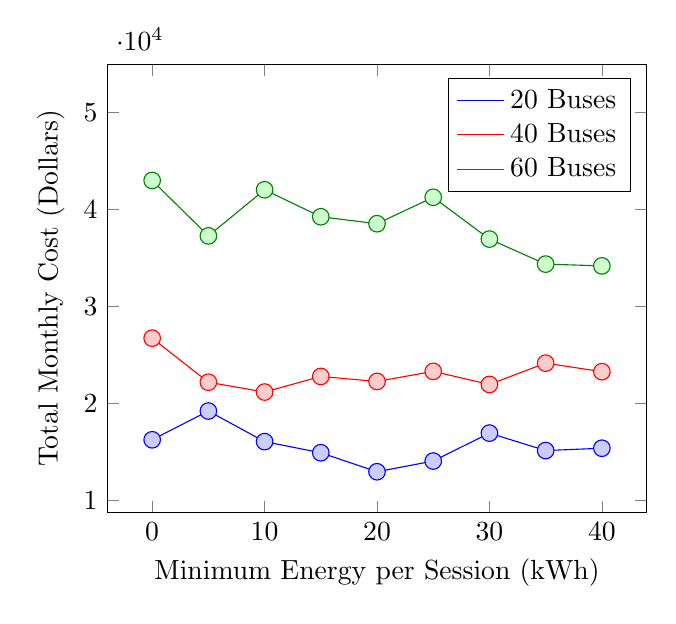
\begin{tikzpicture}
\begin{axis}[xlabel=Minimum Energy per Session (kWh), ylabel=Total Monthly Cost (Dollars), ymax=55000, legend pos=north east]
	\addplot[blue] coordinates {
		(0, 16256.21)   
	  (5, 19221.75)  
		(10,16068.21)  
		(15,14919.20)  
		(20,12958.06)  
		(25,14062.05)  
		(30,16946.17)  
		(35,15143.95)  
		(40,15386.03)};
\addplot[red] coordinates {
		(0, 26738.71)
		(5, 22196.87) 
	  (10,21180.43)
		(15,22789.78)
		(20,22273.05)
		(25,23312.12)
		(30,21963.29)
		(35,24164.56)
		(40,23282.00)};
\addplot[green!50!black] coordinates {
		(0, 43007.78)
		(5, 37289.58)
	  (10,42044.81)
		(15,39261.70)
		(20,38546.15)
		(25,41271.99)
		(30,36959.39)
		(35,34377.97)
		(40,34195.29)}; 
\addplot[blue!20, draw=blue, only marks, mark size=3pt] coordinates {
		(0, 16256.21)   
	  (5, 19221.75)  
		(10,16068.21)  
		(15,14919.20)  
		(20,12958.06)  
		(25,14062.05)  
		(30,16946.17)  
		(35,15143.95)  
		(40,15386.03)};
\addplot[red!20, draw=red, only marks, mark size=3pt] coordinates {
		(0, 26738.71)
		(5, 22196.87) 
	  (10,21180.43)
		(15,22789.78)
		(20,22273.05)
		(25,23312.12)
		(30,21963.29)
		(35,24164.56)
		(40,23282.00)};
\addplot[green!20, draw=green!50!black, only marks, mark size=3pt] coordinates {
		(0, 43007.78)
		(5, 37289.58)
	  (10,42044.81)
		(15,39261.70)
		(20,38546.15)
		(25,41271.99)
		(30,36959.39)
		(35,34377.97)
		(40,34195.29)}; 
\legend{20 Buses, 40 Buses, 60 Buses} 
\end{axis}
\end{tikzpicture}
\caption{Cost comparison of different degragmentation thresholds in a pro-schedule optimization scheme.}
\label{fig:results:costDefragmentationProTime}
\end{figure}


	
	

\section{Conclusions}
In summary, this paper proposes a method to compute cost-oriented charge schedules for large numbers of battery electric buses by dividing the charge problem into several sub-problems which focus on energy placement, group separation, defragmentation, bus-to-charger assignment, and cost optimization. 

\section*{Acknowledgment}This material is based in part upon work supported by the National Science Foundation through the ASPIRE Engineering Research Center under Grant No. EEC-1941524, the Department of Energy through a prime award with ABB under Grant No. DE-EE0009194, and PacifiCorp under contract number 3590. Any opinions, findings, and conclusions or recommendations expressed in this material are those of the authors and do not necessarily reflect the views of the National Science Foundation, the Department of Energy, or Pacificorp.
%\newpage 
\onecolumn
\newcommand\mybar{\kern1pt\rule[-\dp\strutbox]{.8pt}{\baselineskip}\kern1pt}
\newcommand{\coloredhline}{\arrayrulecolor{gray!20} \hline \\[0.01in]\arrayrulecolor{black}}
\newcommand{\myendline}{\\ \coloredhline}
\label{tab:paperVariables}
\centering
\begin{supertabular}{b{0.06\textwidth} m{0.3\textwidth} m{0.09\textwidth} m{0.06\textwidth} m{0.3\textwidth} m{0.09\textwidth}}
	\toprule%----------------------------------------------------------------------------
	\textbf{Variable} & \textbf{Description} & \textbf{Range} & \textbf{Variable} & \textbf{Description} & \textbf{Range}\\
	\toprule%-----------------------------------------------------------------------------
	\multicolumn{6}{l}{Indices} \myendline
	i & Bus index     & $\mathbb{N}$ & j & Time Index & $\mathbb{N}$\\ \myendline
	k & Charger index & $\mathbb{N}$ & r & Route Index \\ \myendline
  m & group index   & $\mathbb{N}$ &   &             \\[0.15in]
	\hline \\[-5pt]
	\multicolumn{6}{l}{Optimal Solution | Formulation} \\[-9pt]\myendline
	$n_{\text{bus}}$&\parbox{0.3\textwidth}{The number of buses in the optimization framework.}                                                           & $\mathbb{Z}$            & $n_{\text{time}}$                      &\parbox{0.3\textwidth}{ The number of time indices in a day.                                                                                 }      & $\mathbb{Z}^+$ \\\myendline
	$b_{p(i,j)}$   & \parbox{0.3\textwidth}{The average power consumed by bus $i$ during time period $j$.}                                                                              & $\mathbb{R}$           & $t_j$         &\parbox{0.3\textwidth}{ The time at time index $j$. This paper also refers to the period of time from $t_j$ to $t_{j+1}$ as ``period $t_j$''.}      & $\mathbb{R}$\\\myendline 
	$\bm{b}$       & \parbox{0.3\textwidth}{A vector containing each value for $b_{p(i,j)}$.}                                                                                          & $\mathbb{R}^{n_{\text{bus}}\cdot n_{\text{time}}}$           & 	$\mathcal{\tilde{A}}$  & \parbox{0.3\textwidth}{The complement of $\mathcal{A}$.}                                                                        & $i\times j$\\\myendline 
	$\mathcal{A}$  & \parbox{0.3\textwidth}{The set of all $i\times j$ elements where bus $i$ can charge at time index $j$}                                  & $i\times j$             & $p_{\text{max}}$ &\parbox{0.3\textwidth}{The maximum power a bus charger can deliver to a bus in kW. This paper assumes a value of 350 for most examples and results.} & $\mathbb{R}^+  $\\[0.5in]
	\hline \\[-0.07in]
	\multicolumn{6}{l}{Optimal Solution | Battery} \\[-9pt] \myendline
	$h_{\text{min}}$ & The minimum allowable state of charge                           & $\left ( 0,h_{\text{max}} \right )$                & $h_{\text{max}}$  & The maximum state of charge                                                   & $\mathbb{R}^+$                                     \\ \myendline 
	$\eta_i$         & The beginning state of charge for bus $i$                       & $\left ( h_{\text{min}}, h_{\text{max}} \right )$  & $h(ij)$           & The state of charge for bus $i$ at time $t_j$. & $\left ( h_{\text{min}}, h_{\text{max}} \right )$\\ \myendline
	$\Delta T$       & The change in time from $t_j$ to $t_{j+1}$                      &$\mathbb{R}^+ $  & $\bm{h}$             & A vector containing all state of charge values.                                        & $\mathbb{R}_+^{n_{\text{bus}}\cdot n_{\text{time}}}$                                   \\ \myendline
	$\delta(ij)$     & The battery discharge for bus $i$ during time period $j$.               & $\mathbb{R}_+$                                     & $h(i,\text{end})$& Bus $i$'s final state of charge.                                              & $\left ( h_{\text{min}}, h_{\text{max}} \right )$\\[0.3in]
	\hline \\[-0.07in]
	\multicolumn{6}{l}{Optimal Solution | Cumulative Load Management} \\[-9pt] \myendline 
	$n_{\text{charger}}$             & The time index for the start of bus $i$'s $j^{\text{th}}$ stop                                                    & $\mathbb{Z}_+$                   & $p_c(j)$            & The average power consumed by all buses during time period $j$. & $\mathbb{R}$                    \\ \myendline
	$\bm{p_c}$                       & A vector containing all values of $p_c(j)$.                                                                       & $\mathbb{R}_{+}^{n_{\text{time}}}$                   & $J_{\text{thrash}}$          & A secondary objective function which penalizes multiple plug-in instances per charge session.& $\mathbb{R}_+$ \\ \myendline
	$g(i,j)$                         & A slack variable used to compute the absolute value of $\lvert b_{p(i,j)} - b_{p(i,j-1)}\rvert$ & $\mathbb{R}_+$& & &                \\[0.3in] 
	\hline \\[-0.07in]
	\multicolumn{6}{l}{Optimal Solution | Objective}  \\[-9pt] \myendline
	$\mu_{\text{e-on}}$         & On-Peak Energy Rate                                                            & $\mathbb{R}_+$                                & $\mu_{\text{e-off}}$       & Off-Peak Energy Rate                                                                                     & $\mathbb{R}_+$                 \\ \myendline
	$\mu_{\text{p-on}}$         & On-Peak Demand Power Rate                                                      & $\mathbb{R}_+$                                & $\mu_{\text{p-all}}$       & Facilities Power Rate                                                                                    & $\mathbb{R}_+$                 \\ \myendline
	$\mathcal{S}_{\text{on}}$   & The set of on-peak time indices                                                & \scalebox{0.9}{$\{1,...,n_{\text{time}}\}$}   & $p_{\text{demand}}$        & Maximum average power during on-peak periods                                                             & $\mathbb{R}$                 \\ \myendline
	$p_{\text{facilities}}$     & Maximum average power over all time instances.                                 & $\mathbb{R}_+$                                & $p_t(j)$                   & The total average power co nsumed by both the bus chargers and the uncontrolled loads.                    & $\mathbb{R}_+^{n_{\text{time}}}$  \\ \myendline
	$u(j)$                      & The average power over time $j$ consumed by the uncontrolled loads             & $\mathbb{R}_+^{n_{\text{time}}}$            & $\bm{p}_t$                 & a vector containing $p_t(i)$ for all $i$.                                                                  & $\mathbb{R}_+^{n_{\text{time}}}$ \\ \myendline 
	$e_{\text{on}}$             & The total amount of energy consumed by the bus chargers and uncontrolled loads during off-peak hours.& $\mathbb{R}_+$                              & $e_{\text{off}}$             & The total energy consumed by the bus chargers and uncontrolled loads during on-peak hours.               & $\mathbb{R}_+$ \\ \myendline 
	$J_{\text{cost}}$           & The section of the objective function pertaining to the fiscal expense of charging buses. & $\mathbb{R}$                & $J_{\text{all}}$               & The expression for the complete objective function. & $\mathbb{R}$ \\[0.3in]
	\hline \\[-0.07in] 
	\multicolumn{6}{l}{Scalability}  \\[-9pt] \myendline
	$n_{\text{group}}$         & The number of groups in which to divide the buses and available chargers in preparation for the $p_4$, $p_5$, and $p_6$.                                                           & $\mathbb{Z}_+$                                & $n_{\text{charger}}^m$      & The number of chargers assigned to group $m$.             & $\mathbb{Z}_+$ \myendline
  $n_{\text{bus}}^m$         & The number of buses in group $m$.                                                                                      &$\mathbb{Z}_+$ & $p(j,m)$ & The total power used during time index $j$ by all buses in group $m$. & $\mathbb{R}_+$      \myendline
  $\beta(i,m)$               & A binary selector variable which is one when bus $i$ is in gropu $m$ and zero otherwise.                               &$\{0,1\}$      & $n_{\text{charger}}^m$ & The number of chargers assigned to group $m$            & $\mathbb{Z}_+$      \myendline
  $\phi(i,i')$                  & The inner product of the optimal charge schedules for buses $i$ and $i'$ respectively.                                 &$\mathbb{R}_+$&$v(i,i',g)$ & A variable that is $w(i,i')$ when buses $i$ and $i'$ are in group $g$ and zero otherwise. & $\mathbb{Z}_+$    \myendline
  $M_s$                      & The maximum value for $\phi(i,i')$.                                                                                       &$\mathbb{R}_+$&$J_{\text{select}}$ & The objective function for the group-selection problem & $\mathbb{R}_+$ \\[0.3in]
	\hline \\[-0.07in] 
	\multicolumn{6}{l}{De-Fragmentation}  \\[-9pt] \myendline
	$\theta(i,r)$& A binary variable which is one when charge session $r$ from bus $i$ will be used in a defragmented solution. & $\{0,1\}$ & $\rho(i,r)$ & A vector whose elements are equal to $\Delta T$ during time indices when bus $i$ is charging during charge session $r$ and zero otherwise.  & $\mathbb{R}^{n_{\text{time}}}$\\ \myendline
  $\psi(i,j)$& The minimum allowable energy delivered to bus $i$ during charge session $r$ where the session in question is considered ``active''. & $\mathbb{R}$& $\omega$	& The minimum allowable energy for any charge session. & $\mathbb{R}$ \\ \myendline
	$e_{\text{max}}$ & The maximum allowable energy delivered in any session.                                                                        & $\mathbb{R}$& & & \\[0.3in] 
	\hline \\[-0.07in]
	\multicolumn{6}{l}{Charge Schedules}  \\[-9pt] \myendline
	$a(i,r)$ & The beginning of the allowable charge interval for bus $i$'s $r^{\text{th}}$ charge session. & $\mathbb{R}_+$ & $b(i,r)$ & The commanded start time for bus $i$'s $r^{\text{th}}$ charge session& $\mathbb{N}$\\ \myendline
	$f(i,r)$ & The commanded end time for bus $i$'s $r^{\text{th}}$ charge session. & $\mathbb{R}_+$ & $d(i,r)$ & The end time of the allowable charge interval for bus $i$'s $r^{\text{th}}$ charge session. & $\mathbb{R}_+$ \\\myendline
	$\sigma(i,r,k)$& A selector variable which is one when bus $i$ charges at charger $k$ for session $r$. & $\{0,1\}$ & $M$ & The number of seconds in a day & $\mathbb{Z}_+$ \\ \myendline
	\scalebox{0.8}{$l(i,r,i',r')$} & A selector variable which is one when bus $i$ charges before bus $i'$ during the $r$ and $r'$ sessions respectively. & $\{0,1\}$& & & \\[0.3in]
	\hline \\[-0.07in]	
	\multicolumn{6}{l}{Optimizing Charge Schedules}  \\[-9pt] \myendline
	$c(s,i,r)$ & The start time for bus $i$'s $r^{\text{th}}$ charge session.  & $\mathbb{R}$ & $c(f,i,r)$& The stop time for bus $i$'s $r^{\text{th}}$ charge session. & $\mathbb{R}$ \\ \myendline
	$c(a,i,r)$ & The arrival time of bus $i$ for charge session $r$.           & $\mathbb{R}$ & $c(d,i,r)$& The departure time for bus $i$ after having completed the $r^{\text{th}}$ charge session& $\mathbb{R}$ \myendline
	$J_{\text{window}}$ & The loss function which drives charge windows to the desired length.& $\mathbb{R}$ & & & \\[0.3in]
	\hline \\[-0.07in]
	\multicolumn{6}{l}{Multi-Rate Charging}  \\[-9pt] \myendline
	$x(i,j)$ & The final charge schedule for bus $i$ at time $j$, yielding the power at which bus $i$ will charge.& $\mathbb{R}_+$ & $z(j)$ & The total power used by all buses at time $j$. $\mathbb{R}_+$ \\ \myendline
  $\gamma(i,d)$ & A binary vector which is one at all time steps where bus $i$ charges during charge session $d$. &$\{0,1\}^{n_{\text{time}}}$& $e(i,r)$               &The amount of energy to be delivered to bus $i$ during charge session $r$.        &$\mathbb{R}_+$            \\ \myendline
  $J_{\text{multi-rate}}$ & The objective function over which we minimize to solve the multi-rate section of the bus charge problem. & $R_+$& &  &             \\[0.3in] 
	\hline \\[-0.07in]
	%
\end{supertabular}
\twocolumn

\printbibliography
\end{document}


